
\documentclass[a4paper,12pt,twoside]{report}
\usepackage[left=2cm,right=2cm,top=2cm,bottom=3cm]{geometry}
\usepackage{graphicx}
\usepackage{verbatim}
\usepackage{latexsym}
\usepackage{setspace}
\usepackage{mathtools}
\usepackage[english,greek]{babel}
\usepackage[utf8x]{inputenc}
\usepackage[LGR, T1]{fontenc}


\pagestyle{empty}

\setlength{\parskip}{2ex plus 0.5ex minus 0.2ex}
\setlength{\parindent}{0pt}

\makeatletter  %to avoid error messages generated by "\@". Makes Latex treat "@" like a letter

\linespread{1.5}
\def\submitdate#1{\gdef\@submitdate{#1}}

\def\maketitle{
  \begin{titlepage}{
    %\linespread{1.5}
    \Large Αριστοτέλειο Πανεπιστήμιο Θεσσαλονίκης \\
    %\linebreak
    Πολυτεχνική Σχολή \\
    %\linebreak
    Τμήμα Ηλεκτρολόγων Μηχανικών και Μηχανικών Η/Υ
    \rm
    \vskip 1.5in
    \Large \bf \@title \par
  }
  \vskip 3.5in
  \par
  {Εκπόνηση: \\ \vskip 0.07in \Large \@author}
  \linebreak
  \par
  {Επίβλεψη: \\ \vskip 0.05in \Large Νικόλαος Πιτσιάνης \\ 
  			\vskip 0.07in Νίκος Σισμάνης}
  \vskip 1in
  \par
  Με την εκπόνηση της εν λόγω διπλωματικής εργασίας ολοκληρώνεται ο κύκλος των προπτυχιακών μου σπουδών αποκτώντας δίπλωμα Ηλεκτρολόγου Μηχανικού και Μηχανικού Η/Υ απο το Αριστοτέλειο Πανεπιστήμιο Θεσσαλονίκης.  \\
  \vfil
  \end{titlepage}
}

\def\titlepage{
  \newpage
  \centering
  \linespread{1}
  \normalsize
  \vbox to \vsize\bgroup\vbox to 9in\bgroup
}
\def\endtitlepage{
  \par
  \kern 0pt
  \egroup
  \vss
  \egroup
  \cleardoublepage
}

\def\abstract{
  \begin{center}{
    \large\bf Περίληψη}
  \end{center}
  \small
  %\def\baselinestretch{1.5}
  \linespread{1.5}
  \normalsize
}
\def\endabstract{
  \par
}

\newenvironment{acknowledgements}{
  \cleardoublepage
  \begin{center}{
    \large \bf Ευχαριστίες}
  \end{center}
  \small
  \linespread{1.5}
  \normalsize
}{\cleardoublepage}
\def\endacknowledgements{
  \par
}

\newenvironment{dedication}{
  \cleardoublepage
  \begin{center}{
    \large \bf Αφιέρωση}
  \end{center}
  \small
  \linespread{1.5}
  \normalsize
}{\cleardoublepage}
\def\enddedication{
  \par
}

\def\preface{
    \pagenumbering{roman}
    \pagestyle{plain}
    \doublespacing
}

\makeatother  %to avoid error messages generated by "\@". Makes Latex treat "@" like a letter


\begin{document}
\title{\LARGE {\bf ΜΗ ΓΡΑΜΜΙΚΗ ΜΕΙΩΣΗ ΔΙΑΣΤΑΣΕΩΝ \\ 
	    ΜΕ ΤΗ ΧΡΗΣΗ ΤΟΥ ΑΛΓΟΡΙΘΜΟΥ 
	    \textlatin{LOCALLY LINEAR EMBEDDINGS} ΚΑΙ \\
	    ΣΤΟΧΟ ΤΗ ΒΕΛΤΙΩΣΗ ΤΟΥ ΠΟΣΟΣΤΟΥ ΤΑΞΙΝΟΜΗΣΗΣ \\ 
	    ΣΕ ΕΦΑΡΜΟΓΕΣ ΕΞΟΡΥΞΗΣ ΓΝΩΣΗΣ ΚΑΙ ΜΗΧΑΝΙΚΗΣ ΜΑΘΗΣΗΣ} \\
 \vspace*{16mm}
}

\author{Πέτρος Κατσιλέρος}
\submitdate{ΜΑΡΤΙΟΣ 2016}

\maketitle

\preface

\pagenumbering{arabic}


%\addcontentsline{toc}{chapter}{Abstract}

\begin{abstract}
\par
Στα πλαίσια της εργασίας αυτής διερευνήθηκε η συμπεριφορά και η απόδοση του αλγορίθμου <<Τοπική Γραμμική Ενσωμάτωση>>\cite{lle} στο πεδίο της Αναγνώρισης Προτύπων. Ο αλγόριθμος ανήκει στην ευρύτερη κατηγορία <<Αλγόριθμοι Μείωσης των Διαστάσεων>> με τους οποίους μπορούμε να επιτύχουμε μείωση των παραμέτρων οι οποίες προσδιορίζουν κάποιο συγκεκριμένο πρόβλημα. Οι βασικοί μας στόχοι μέσω αυτής της διαδικασίας είναι αρχικά η συμπίεση της πληροφορίας, δηλαδή η δυνατότητα να εκφράσουμε την πληροφορία των αρχικών μας δεδομένων με ένα υποσύνολο της, με τις ελάχιστες δυνατές απώλειες. Επίσης μπορούμε να επιτύχουμε τεράστια μείωση της υπολογιστικής πολυπλοκότητας αλλά και της διαθέσιμης μνήμης που απαιτούνται για την προσπέλαση,αποθήκευση και μετέπειτα επεξεργασία των δεδομένων. Τέλος υπάρχουν περιπτώσεις στις οποίες θέλουμε να απομακρύνουμε απο τα δεδομένα μας, στοιχεία τα οποία αποτελούν θόρυβο και επιδρούν αρνητικά στην εξαγωγή ορθού συμπεράσματος ταξινόμησης. 
\par
Πιο συγκεκριμένα έγινε εφαρμογή της διαδικασίας μείωσης των διαστάσεων μέσω του αλγορίθμου <<Τοπική Γραμμική Ενσωμάτωση>>\cite{lle} σε τρία σετ δεδομένων. Τα δύο πρώτα περιέχουν εικόνες με ψηφία-αριθμούς και είναι τα \textlatin{MNIST}\cite{16} και \textlatin{Google Streen View House Numbers}\cite{12}. Το τρίτο είναι το \textlatin{Arcene}\cite{15} και περιέχει δεδομένα απο τον χώρο της Ιατρικής και συγκεκριμένα πρόκειται για δεδομένα απο ασθενείς με σκοπό την πρόβλεψη εμφάνισης κάποιας μορφής καρκίνου. Στα πρώτα δύο ο στόχος μας είναι να γίνει σωστή αναγνώριση κάθε ψηφίου. 
\par
Ο τελικός σκοπός είναι να προσδιορίσουμε με ακρίβεια κατά πόσο μπορούμε να επιτύχουμε συμπίεση της πληροφορίας και τι επιδράσεις θα έχει αυτό στην διαδικασία της ταξινόμησης των δεδομένων σε κλάσεις. Μέσα απο τα πειράματα λοιπόν έγινε προσπάθεια να διερευνηθεί τόσο η αποτελεσματικότητα του αλγορίθμου στα διαφορετικά σετ δεδομέναν αλλά και την επίδραση που έχουν οι παράμετροί του στην επίλυση κάθε προβλήματος χωριστά. Ως μετρική αξιολόγησης της αποτελεσματικότητας του αλγορίθμου χρησιμοποιήθηκε η σύγκριση μεταξύ του σφάλματος ταξινόμησης πρίν και μετά την διαδικασία μείωσης των διαστάσεων.
\par
Πολύ σημαντικό εύρημα της εν λόγω δουλειάς πέραν των πολύ ικανοποιητικών αποτελεσμάτων μετά την μείωση των διαστάσεων είναι η παρουσίαση δύο νέων μεθόδων, οι οποίες αποτελούν παραλλαγές του αλγορίθμου <<Τοπική Γραμμική Ενσωμάτωση>>\cite{lle}. Με την πρώτη μέθοδο γίνεται εφικτή η χρήση του αλγορίθμου σε προβλήματα ταξινόμησης όπου τα αποτελέσματα θα πρέπει να δίνονται σε <<πραγματικό χρόνο>>, μειώνοντας παράλληλα και την πολυπλοκότητα εκτέλεσης του αλγορίθμου. Με την δεύτερη μέθοδο μειώνεται δραματικά το πολύ μεγάλο υπολογιστικό κόστος που απαιτεί ο αλγόριθμος κατά την εκτέλεσή του. Τέλος, πολύ σημαντικό στοιχείο αποτελεί το γεγονός ότι οι δύο αυτές μέθοδοι μπορούν να συνδιαστούν μεταξύ τους έχοντας έτσι πολλαπλή μείωση της πολυπλοκότητας και άμεση εξαγωγή των αποτελεσμάτων ταξινόμησης.  


\end{abstract}


\cleardoublepage

%\addcontentsline{toc}{chapter}{Acknowledgements}

\begin{acknowledgements}

\par Με την ολοκλήρωση αυτής της διπλωματικής εργασίας θα ήθελα καταρχήν να ευχαριστήσω τον επίκουρο καθηγητή του τμήματός Ηλεκτρολόγων Μηχανικών και Μηχανικών Η/Υ του Αριστοτελείου Πανεπιστημίου Θεσσαλονίκης κ.Νικόλαο Πιτσιάνη ο οποίος μου έδωσε το ερέθισμα, απαραίτητες χρήσιμες συμβουλές αλλά και πόρους ώστε να μπορέσω να ολοκληρώσω την έρευνα για το συγκεκριμένο θέμα. Επίσης ένα μεγάλο ευχαριστώ στον υποψήφιο διδάκτορα του τμήματος Νίκο Σισμάνη για την καθοδήγηση του καθ' όλη την διάρκεια εκπόνησης της εργασίας μου αυτής. 

\par Τέλος, ένα πολύ θερμό και μεγάλο ευχαριστώ στους γονείς μου οι οποίοι με στήριξαν τόσο οικονομικά όσο και ψυχολογικά όλα αυτά τα χρόνια ώστε να μπορέσω να αποκτήσω το δίπλωμά μου. Στο σημείο αυτό δεν θα μπορούσα να παραλείψω τον σκύλο μου,την κοπέλα και τους φίλους μου διότι ο καθένας ξεχωριστά και με τον τρόπο του βοήθησαν στην αντιμετώπιση των δυσκολιών που συνάντησα καθ' όλη την διάρκεια των σπουδών μου.

\begin{flushright}
Κατσιλέρος Πέτρος \\
Θεσσαλονίκη, Μάιος 2016
\end{flushright}

\end{acknowledgements}


\cleardoublepage

\begin{dedication}
\par
Αφιερώνω την διπλωματική αυτή εργασία πρωτίστως στον εαυτό μου για τον κόπο μου όλα αυτά τα χρόνια ώστε να μπορέσω να αποκτήσω το δίπλωμα Ηλεκτρολόγου Μηχανικού και Μηχανικού Η/Υ και κατά δεύτερον στους γονείς μου οι οποίοι με στήριξαν ανελλιπώς και με κάθε τρόπο σε όλη αυτή την πορεία.
\begin{flushright}
Κατσιλέρος Πέτρος \\
Θεσσαλονίκη, Μάρτιος 2016
\end{flushright}
\end{dedication}


\clearpage

%\narrowlinespacing

\vspace*{4mm}
\begin{flushleft}
\textbf{Τι φέρνει μια χαλώνα απο την Κίνα ...}
\end{flushleft}

\vspace*{2mm}
\begin{center}
\textbf{\Large Το πτυχίο μου !!!}
\end{center}

%\normallinespacing


\cleardoublepage    
\tableofcontents

\cleardoublepage
\listoftables

\cleardoublepage
\listoffigures

\cleardoublepage


\chapter{Εισαγωγή}

\section{Αναγνώριση προτύπων και μηχανική μάθηση}
\par
Αναγνώριση προτύπων καλείται η επιστημονική περιοχή που έχει στόχο την ταξινόμηση αντικειμένων σε κατηγορίες ή κλάσεις. Ανάλογα με την κάθε εφαρμογή τα δεδομένα μπορεί να είναι είτε εικόνες, είτε σήματα είτε οποιοδήποτε άλλο σετ δεδομένων χρειάζεται για κάποιο λόγο να ταξινομηθεί. Στις μέρες μας η ανάγκη διαχείρισης αλλά και ανάκτησης πληροφοριών μέσω ηλεκτρονικών υπολογιστών αποκτά τεράστια σπουδαιότητα καταρχήν διότι ο όγκος των πληροφοριών αυξάνεται ραγδαία με ρυθμό αδύνατο να διαχειριστεί ο άνθρωπος και επίσης διότι η ανάπτυξη της τεχνολογίας μας παρέχει πολύ ισχυρά υπολογιστικά συστήματα με τη χρήση των οποίων μπορούμε να δημιουργήσουμε πολύπλοκα μοντέλα εξόρυξης γνώσης . 
\par
Αντίστοιχοι κλάδοι στους οποίους έχει τεράστια σημασία η αναγνώριση προτύπων είναι οι επιστημονικοί κλάδοι της Ιατρικής, της Βιολογίας, ο χώρος των αγορών και των επιχειρήσεων και τέλος η διαχείριση και η εξόρυξη γνώσης απο τον τεράστιο όγκο της πληροφορίας που είναι διαθέσιμος στο διαδίκτυο. Φυσικά η αναγνώριση προτύπων είναι ένα πολύ σημαντικό μέρος του κλάδου της μηχανικής μάθησης σε ρομποτικά/υπολογιστικά συστήματα.
\par
Η υπολογιστική όραση για παράδειγμα είναι αντικείμενο ιδιαίτερα χρήσιμο τόσο στον χώρο της ρομποτικής όσο σε αυτόν της ιατρικής αλλά και προφανώς της βιομηχανίας. Τέτοιου είδους εφαρμογές έχουν εισέλθει πολύ δυναμικά στην καθημερινότητά μας τα τελευταία χρόνια. Συγκεκριμένα στον χώρο της βιομηχανίας υπάρχουν συστήματα τα οποία επιβλέπουν μέσω μια κάμερας την γραμμή παραγωγής καθώς και ρομπότ τα οποία μεταφέρουν και συναρμολογούν αντικείμενα. Eπίσης υπάρχουν εφαρμογές οι οποίες αναγνωρίζουν για παράδειγμα πρόσωπα τραβώντας μια εικόνα με το κινητό μας τηλέφωνο. Τέλος στον χώρο της αυτοκινητοβιομηχανίας δεν είναι λίγες αντίστοιχες εφαρμογές οι οποίες έχουν συμβάλει δυναμικά στην αυτόνομη οδήγηση αλλά και στην προειδοποίηση για εμπόδια κλπ.
\par
Ιδιαίτερη έμφαση αξίζει να δωθεί στην εξόρυξη γνώσης σε κλάδους όπως στη βιολογία αλλά και στην ιατρική. Για παράδειγμα η πρόβλεψη εμφάνισης ασθενειών όπως ο καρκίνος μέσω αναγνώρισης συγκεκριμένων μοτίβων σε εικόνες απο μαγνητικό τομογράφο, η μελέτη της αλύσίδας του γεννετικού υλικού αλλά και ο χώρος των εγχειρίσεων υψηλής ακρίβειας με τη χρήση της ρομποτικής.

\section{Ερεθίσματα απο τον τρόπο λειτουργίας του ανθρώπινου εγκεφάλου}
\par
Απο μελέτες που έχουν γίνει για την λειτουργία του ανθρώπινου εγκεφάλου γνωρίζουμε ότι για οποιοδήποτε σύνολο μετρήσεων προέρχεται για παράδειγμα είτε απο την όραση μας είτε απο την ακοή μας ο εγκέφαλός μας μετασχηματίζει το σύνολο των δεδομένων αυτών σε ένα νέο σύνολο χαρακτηριστικών. Με τον τρόπο αυτό, επιλέγοντας προφανώς κάθε φορά τα κατάλληλα χαρακτηριστικά, επιτυγχάνεται τεράστια συμπίεση του όγκου της πληροφορίας σε σύγκριση με τα αρχικά δεδομένα εισόδου. Αυτο σημαίνει λοιπόν ότι το μεγαλύτερο μέρος της πληροφορίας για παράδειγμα μια σκηνής που βλέπουμε και στην οποία θέλουμε να αναγνωρίσουμε τα αντικείμενα που περιέχονται, συμπιέζεται σε έναν πολύ μικρό αριθμό χαρακτηριστικών. Η παραπάνω διαδικασία χαρακτηρίζεται ως τεχνική μείωσης διάστασης γνωστή στην βιβλιογραφία με τον όρο \textlatin{Dimensionality Reduction}.
\par
Ας πάρουμε για παράγειγμα τον κλάδο της υπολογιστικής όρασης ο οποίος αποτελεί και αντικείμενο μελέτης της εν λόγω εργασίας και ας αναρωτηθούμε το εξής: Πόσο δύσκολο είναι για κάποιον απο εμάς να ανγνωρίσει κάποιο νούμερο αποτυπωμένο σε μια εικόνα; Η προφανής απάντηση είναι καθόλου. Και αυτή είναι μια πολύ σωστή απάντηση, διότι για τον ανθρώπινο εγκέφαλο το να καταλάβει οτι το ψηφίο το οποίο βρίσκεται στην εικόνα είναι για παράδειγμα το 1 και όχι το 9 είναι ένα πολύ απλό πρόβλημα. 
\par
Πιο συγκεκριμένα βλέποντας μια οποιαδήποτε σκηνή ο ανθρώπινος εγκέφαλος προσπαθεί να εντοπίσει σημεία ενδιαφέροντος τα οποία αποτελούν χαρακτηριστικά σημεία της. Τέτοια μπορεί να είναι πολύ έντονες αλλαγές στην φωτεινότητα όπως για παράδειγμα γωνίες, κενά ή τρύπες. Στην συνέχεια εντοπίζει πιο σύνθετες γεωμετρίες όπως ευθείες ή καμπύλες γραμμές και τέλος προσδιορίζει πιο ολοκληρωμένες δομές τρισδιάστατων αντικειμένων. Το ίδιο ακριβώς γίνεται και στην παραπάνω περίπτωση με το ψηφίο. Εντοπίζουμε αρχικά οτι το μοτίβο του ψηφίου 1 είναι πολύ κοντά σε αυτά των ψηφίων εφτά και τέσσερα αλλά σε καμιά περίπτωση δεν θα λέγαμε οτι έχει τρομερές ομοιότητες με αυτό του δύο ή του οχτώ για παράδειγμα. 
\par
Το παραπάνω παράδειγμα είναι ένα πολύ απλό δείγμα του τρόπου με τον οποίο ο ανθρώπινος εγκέφαλος προσπαθεί με κάθε τρόπο να ελαχιστοποιήσει τις παραμέτρους που πρέπει να εκτιμήσει. Φυσικά αν αναλογιστούμε ένα ρεαλιστικό περίπλοκο πρόβλημα της καθημερινότητάς μας θα δούμε οτι απαιτούνται πολύ πιο σύνθετοι υπολογισμοί και θα πρέπει να συνδιάσουμε ένα πλήθος απο παραμέτρους ώστε τελικά να καταλήξουμε στο τελικό συμπέρασμα για κάποια απόφαση. Σε κάθε περίπτωση όμως γίνεται τεράστια συμπίεση της αρχικής πληροφορίας μέσω τεχνικών μείωσης διαστάσεων ώστε να ελαχιστοποιηθούν οι παράμετροι που πρέπει να υπολογιστούν και προφανώς να επιταχυνθεί η διαδικασία εξαγωγής της τελικής μας απόφασης.
\par Το γεγονός αυτό και δεδομένου οτι το όραμα της επιστημονικής κοινότητας των μηχανικών που ασχολούνται με την μηχανική μάθηση και την εξόρυξη γνώσης είναι να δημιουργηθεί ένα μοντέλο αντίστοιχο με αυτό του ανθρώπινου εγκεφάλου δεν θα μπορούσε να τους αφήσει αδιάφορους ώστε να μελετήσουν και να αναπτύξουν αντίστοιχους αλγορίθμους με σκοπό να εφαρμοστούν σε μοντέλα εξόρυξης γνώσης.


\subsection{Μάθηση με επίβλεψη - χωρίς επίβλεψη - με ημιεπίβλεψη}
\par
Ένα πολύ εύλογο ερώτημα το οποίο προκύπτει απο την παραπάνω ανάλυση είναι πως ο ανθρώπινος εγκέφαλος έχει μάθει και τελικώς έχει αποθηκεύσει το σύνολο αυτών των μοντέλων για τον κάθε αριθμό ή για οποιοδήποτε άλλο αντικείμενο ή μοτίβο μπορεί να αναγνωρίσει με τόσο μεγάλη ταχύτητα και ευκολία. Η απάντηση είναι προφανώς η συνεχής εκπαίδευση και η διαρκής υπενθύμιση των συγκεκριμένων προτύπων.
\par
Πιο συγκεκριμένα ο άνθρωπος απο την μέρα που αρχίζει να αλληλεπιδρά με το περιβάλλον παίρνει διάφορα ερεθίσματα τα οποία καιρό με τον καιρό μαθαίνει να τα ταξινομεί κατάλληλα και να τα χρησιμοποιεί όποτε ξαναεμφανιστούν μπροστά του. Τα ερεθίσματα αυτά είναι είτε εικόνες, είτε ήχοι είτε ερεθίσματα τα οποία μπορεί να προέρχονται απο τις υπόλοιπες αισθήσεις του.
\par
Ο τρόπος με τον οποίο καταφέρνουμε να συγκρατούμε και να μπορούμε να διαχειριστούμε ανα πάσα στιγμή τον τεράστιο όγκο πληροφοριών που βρίσκονται καταχωρημένες στον εγκέφαλό μας είναι ένας συνδιασμός τεχνικών μάθησης και συνεχούς εκπαίδευσης. Οι τεχνικές αυτές στον χώρο της τεχνητής νοημοσύνης αναφέρονται ως τεχνικές μάθησης με επίβλεψη, χωρίς επίβλεψη και με ημιεπίβλεψη. Θα μπορούσε κάποιος αρχικά να υποστηρίξει ότι ο ανθρώπινος εκγέφαλος χρησιμοποιεί κατεξοχήν τεχνικές μάθησης χωρίς επίβλεψη διότι μπορεί να μαθαίνει μόνος του νέα πράγματα. Είναι όμως πραγματικά αυτό το οποίο συμβαίνει; Η απάντηση είναι μάλλον όχι, και αυτό διότι απο την πολύ νεαρή του υλικία ο καθένας μας έχει γύρω του ανθρώπους οι οποίοι προσπαθούν συνεχώς να μας μεταφέρουν γνώση και να μας μάθουν τι βρίσκεται γύρω μας και πως να αλληλεπιδρούμε μεταξύ του. Παρ'όλα αυτά μετά απο κάποιο σημείο ο ανθρώπινος εγκέφαλος αποκτά δυνατότητες με τις οποίες μπορεί αξιολογεί και να μαθαίνει μόνος του πολύ σύνθετα πράγματα αναλύοντάς τα σε απλούστερα προβλήματα τα οποία γνωρίζει ήδη πως να τα διαχειριστεί. Επίσης είναι στην φύση του ανθρώπου να εξερευνεί συνεχώς άγνωστα μονοπάτια και να αναζητεί απαντήσεις σε άγνωστα προβλήματα επιτυγχάνοντας αξιοθαύμαστα αποτελέσματα.
\par
Απο τα παραπάνω καταλήγουμε στο συμπέρασμα ότι ο άνθρωπος χρησιμοποιεί τεχνικές ημιεπίβλεψης για την εκπαίδευση του εγκεφάλου του γεγονός το οποίο του δίνει την δυνατότητα να μπορεί να διαχειριστεί αλλά και να μάθει πολύ σύνθετα μοντέλα. Μέσα απο αυτή την διαδικασία είναι σε θέση με το πέρασμα του χρόνου να δημιουργήσει ένα τεράστιο και πανίσχυρο δίκτυο πληροφοριών, ταξινομημένο με τρόπο τον οποίο δεν μπορούμε ακόμα να εξηγήσουμε και να κατανοήσουμε. Με αυτό το μοντέλο είναι σε θέση ταχύτατα να αποφασίζει που βρίσκεται ο ευρύτερος χώρος της πληροφορίας που θέλει να αντλήσει και στην συνέχεια να αποφασίζει με τεράστια ακρίβεια και ταχύτητα την τελική του απόφαση.   
\par
Το μοντέλο αυτό με το οποίο λειτουργεί ο ανθρώπινος εγκέφαλος είναι αν μη τι άλλο αξιοθαύμαστο και ανεξήγητο. Παρ'όλα είναι πολύ δύσκολο να εφαρμοστεί στον τομέα της τεχνητής νοημοσύνης και αυτό διότι ακόμα δεν είμαστε σε θέση να δώσουμε εξηγήσεις για τον τρόπο λειτουργίας του. Το συνηθέστερο και πιο αποτελεσματικό μέχρι στιγμής μοντέλο το οποίο χρησιμοποιείται στην εξόρυξη γνώσης μέσω ηλεκτρονικών υπολογιστών είναι αυτό της μάθησης με επίβλεψη. Σύμφωνα με το μοντέλο αυτό θα πρέπει αν συλλέξουμε ένα μεγάλο συνήθως όγκο δεδομένων τον οποίο να τροφοδοτήσουμε στην συνέχεια ως είσοδο στο σύστημά μας και με την κατάλληλη μεθοδολογία να το οδηγήσουμε να μάθει συγκεκριμένα μοντέλα τα οποία να μπορεί να χρησιμοποιήσει στην συνέχεια με σκοπό της εξαγωγή κάποιου συμπεράσματος.

\section{Μείωση της διάστασης των δεδομένων}
\par
Στην παραπάνω διαδικασία δεδομένου ότι στις περισσότερες περιπτώσεις έχουμε να αντιμετωπίσουμε πολύ σύνθετα υπολογιστικά προβλήματα ο αριθμός των παραμέτρων που πρέπει να υπολογιστούν είναι σε συγκεκριμένες εφαρμογές απαγορευτικά μεγάλος. Σε κάποιες εφαρμογές το πρόβλημα είναι θέμα χρόνου όπου πρέπει να γίνει μείωση των παραμέτρων ώστε να ελαχιστοποιηθεί ο χρόνος εξαγωγής συμπεράσματος. Σε άλλες είναι θέμα χώρου διότι ένας μεγάλος αριθμός πολυδιάστατων δεδομένων μπορεί να αποτελεί πρόβλημα σε συγκεκριμένες εφαρμογές. Τέλος υπάρχουν περιπτώσεις στις οποίες χρειαζόμαστε την μείωση των διαστάσεων ώστε να διώξουμε εντελώς παραμέτρους οι οποίες επιδρούν σαν θόρυβος και επηρεάζουν αρνητικά την εξαγωγή ορθού συμπεράσματος ταξινόμησης. Προφανώς σε πολλές πρακτικές εφαρμογές επικρατεί ένας συνδυασμός των παραπάνω προβλημάτων.
\par
Αντικείμενο λοιπόν της εν λόγω διπλωματικής εργασίας είναι η διερεύνηση και η χρήση του αλγορίθμου \textlatin{Locally Linear Embeddings} για την μείωση των διαστάσεων σε πρακτικά προβλήματα όπως η αναγνώριση ψηφίων αλλά και η ταξινόμηση ασθενών με βάση το αν πρόκειται να εμφανίζουν κάποιας μορφής καρκίνου ή όχι. Τα αποτελέσματα των πειραμάτων είναι ιδιαίτερα ενθαρυντικά και δείχνουν σε όλες τις περιπτώσεις ότι η μείωση των διαστάσεων επιδρά δραματικά στην μείωση του κόστους των υπολογισμών αλλά και στην αύξηση της σωστής πρόβλεψης λόγω απομάκρυνσης του θορύβου. Επίσης παρουσιάζονται δύο πρακτικές και ρεαλιστικές μέθοδοι εφαρμογής του αλγορίθμου σε πραγματικά προβλήματα απο τις οποίες η πρώτη έρχεται να αντιμετωπίσει το πρόβλημα της πολύ μεγάλης μνήμης που απαιτεί η εκτέλεση του αλγορίθμου και η δεύτερη παρέχει την δυνατότητα για την ταξινόμηση των αποτελεσμάτων και την εξαγωγή συμπεράσματος σε πραγματικό χρόνο. 





\chapter{Μαθηματικό και θεωρητικό υπόβαθρο}
\numberwithin{equation}{section}

\par
Στο κεφάλαιο αυτό παρουσιάζεται το μαθηματικό υπόβαθρο πάνω στο οποίο στηρίζεται η λογική της μείωσης των διαστάσεων. Επίσης γίνεται ανάλυση ορισμένων βασικών τέτοιων μεθόδων ώστε να γίνει καλύτερα αντιληπτό το αποτέλεσμα τέτοιου είδους αλγορίθμων. Το σύνολο της παρακάτω ανάλυσης προέρχεται απο το Κεφάλαιο-6 του συγγράματος << Αναγνώριση Προτύπων, Σ.Θεοδωρίδης και Κ.Κουτρούμπας >> \cite{14}.

\section{Διανύσματα βάσης}
\par
Έστω ότι έχουμε ένα σύνολο δειγμάτων εισόδου με αντίστοιχο διάνυσμα \textlatin{\textbf{x}} διάστασης $N\times1$,
\newline\hspace*{\fill}
$\mathbf{x}^{T} = \begin{bmatrix}
        x(0),\ldots,x(N-1)
        \end{bmatrix}$
\hspace*{\fill}\newline
\newline
Έστω επίσης ορθοκανονικό μητρώο Α, τάξης $Ν\timesΝ$. Τότε ορίζουμε το μετασχηματισμένο διάνυσμα \textlatin{\textbf{y}} του \textlatin{\textbf{x}} ως 
\newline\hspace*{\fill}
\begin{equation}
        \mathbf{y} = \mathbf{A}^{H}\mathbf{x} \equiv \begin{bmatrix}
       \mathbf{a}_{0}^{H} \\
       \vdots \\
       \mathbf{a}_{N-1}^{H} \\
     \end{bmatrix} \mathbf{x}
\end{equation}
\hspace*{\fill}\newline
\newline
Το H δηλώνει τον \textlatin{Hermitian} τελεστή, δηλαδή τον μιγαδικό συζυγή του ανάστροφου. Από τον ορισμό των ορθοκανονικών μητρώων έχουμε   
\newline\hspace*{\fill}
\begin{equation}
        \mathbf{x} = \mathbf{Ay} = \sum_{i=0}^{N-1} y(i)\mathbf{a}_{i}
\end{equation}
\hspace*{\fill}\newline
\newline
Οι στήλες του \textbf{\textlatin{A}}, $\mathbf{a}_{i}=0,1,\ldots,N-1$ καλούνται \textit{διανύσματα βάσης} του μετασχηματισμού. Τα στοιχεία $y(i)$ του $\mathbf{y}$ είναι οι προβολές του διανύσματος $\mathbf{x}$ σε αυτά τα διανύσματα βάσης. Λαμβάνοντας υπόψιν την ιδιότητα της ορθοκανονικότητας μπορούμε να επαληθεύσουμε την παραπάνω διατύπωση υπολογίζοντας το εσωτερικό γινόμενο του $\mathbf{x}$ με το $\mathbf{a}_{j}$. Έχουμε:
\newline\hspace*{\fill}
\begin{equation}
        \langle\mathbf{a}_{j},\mathbf{x}\rangle \equiv \mathbf{a}_{j}^{H}\mathbf{x} = \sum_{i=0}^{N-1} y(i)\langle\mathbf{a}_{j},\mathbf{a}_{i}\rangle = \sum_{i=0}^{N-1} y(i)\delta_{ij} = y(j)
\end{equation}
\hspace*{\fill}

\subsection{Διάνυσμα εικόνας}
\par
Αν πάρουμε για παράδειγμα μια εικόνα, το σύνολο των δειγμάτων εισόδου είναι μια δισδιάστατη ακολουθία $X(i,j), i,j=0,1,\ldots,N-1$, η οποία ορίζει ένα μητρώο $Χ$, τάξεως $Ν\timesΝ$. Σε αυτή την περίπτωση  μπορούμε να μετατρέψουμε την είσοδο αυτή σε ένα διάνυσμα  $\mathbf{x}$ διάστασης $N^{2}$ διατάσσοντας για παράδειγμα τις γραμμές του μητρώου την μία μετά την άλλη έχοντας τελικά \\
\newline\hspace*{\fill}
\begin{equation}
        \mathbf{x}^{T} = \begin{bmatrix}
        X(0,0),\ldots,X(0,N-1),\ldots,X(N-1,0),\ldots,X(N-1,N-1)
        \end{bmatrix}
\end{equation}
\hspace*{\fill}\newline
\newline
Με αυτό τον μετασχηματισμό όμως ο αριθμός των πράξεων που απαιτούνται για τον πολλαπλασιασμό ενός τετραγωνικού μητρώου τάξεως $Ν\timesΝ$ με ένα διάνυσμα $\mathbf{x}$ διαστάσεων $N^{2}\times1$, είναι της τάξης $\mathcal{O}(Ν^{4})$ μέγεθος απαγορευτικό για τις περισσότερες ρεαλιστικές εφαρμογές.

\subsection{Ορθοκανονικά ιδιοδιανύσματα}
\par
Το παραπάνω εμπόδιο μπορεί να ξεπεραστεί αν μετασχηματίσουμε το μητρώο $Χ$ μέσω ενός συνόλου \textit{μητρώων βάσης}. Έστω λοιπόν $U$ και $V$ ορθοκανονικά μητρώα διάστασης $Ν\timesΝ$. Ορίζουμε τότε το μετασχηματισμένο μητρώο $Y$ του $X$ ως
\newline\hspace*{\fill}
\begin{equation}
        Y=U^{H} XV
\end{equation}
\hspace*{\fill}\newline
ή
\newline\hspace*{\fill}
\begin{equation}
        X=UYV^{H}
\end{equation}
\hspace*{\fill}\newline
\newline
Μέσω αυτού του μετασχηματισμού ο αριθμός των πράξεων μειώνεται σε $\mathcal{O}(N^{3})$. Πιο αναλυτικά η παραπάνω εξίσωση θα μπορούσε να γραφεί ως
\newline\hspace*{\fill}
\begin{equation}
        Χ = \sum_{i=0}^{N-1} \sum_{j=0}^{N-1} Y(i,j)\mathbf{u}_{i}\mathbf{v}_{j}^{H}
\end{equation}
\hspace*{\fill}\newline
\newline
όπου $\mathbf{u}_{i}$ είναι τα διανύσματα στήλης του \textlatin{U} και $\mathbf{v}_{j}$ τα διανύσματα στήλης του \textlatin{V}. Η παραπάνω εξίσωση είναι ένα ανάπτυγμα του μητρώου \textlatin{X} ως προς τις $Ν\times2$ εικόνες βάσης. Τέλος κάθε ένα από τα γινόμενα $\mathbf{u}_{i}\mathbf{v}_{j}$ είναι ένα μητρώο $Ν\timesΝ$ \\
\newline\hspace*{\fill}
\begin{equation}
        \mathbf{u}_{i}\mathbf{v}_{j}=\begin{bmatrix}
        u_{i0}v_{j0}^{*}	 &	\ldots  &  u_{i0}v_{jN-1}^{*} 	\\
        \vdots				 &  	\vdots  &  \vdots \\
        u_{iN-1}v_{j0}^{*} &    	\ldots  &  u_{iN-1}v_{jN-1}^{*} \\
        \end{bmatrix}
\end{equation}
\hspace*{\fill}\newline
\newline
Στην περίπτωση κατα την οποία το \textlatin{Y} είναι διαγώνιο τότε έχουμε \\
\newline\hspace*{\fill}
\begin{equation}
        Χ = \sum_{i=0}^{N-1} Y(i,i)\mathbf{u}_{i}\mathbf{v}_{i}^{H}
\end{equation}
\hspace*{\fill}\newline
\newline
με αποτέλεσμα το πλήθος των μητρώων-εικόνων βάσης να μειώνεται σε Ν. Τέλος έπειτα από μερικές πράξεις και τροποποιήσεις μπορούμε να ορίσουμε κάθε στοιχείο $(i,j)$ του μετασχηματισμένου μητρώου ως τον πολλαπλασιασμό κάθε στοιχείου του Χ με τον συζυγή του αντίστοιχου στοιχείου του $Α_{ij}$ και αθροίζοντας όλα τα γινόμενα. Δηλαδή
\newline\hspace*{\fill}
\begin{equation}
        \langle A,B \rangle = \sum_{m=0}^{N-1} \sum_{n=0}^{N-1} A(m,n)^{*}B(m,n)
\end{equation}
\hspace*{\fill}\newline
και τελικά
\newline\hspace*{\fill}
\begin{equation}
        Y(i,j) = \langle A_{i,j},X \rangle
\end{equation}
\hspace*{\fill}\newline

\section{Ο μετασχηματισμός \textlatin{Karhunen-Loeve} - \textlatin{PCA}}
\par
Ο μετασχηματισμός \textlatin{Karhunen-Loeve}\textlatin{\cite{pca}} αξιοποιεί την στατιστική πληροφορία που περιγράφει τα δεδομένα και ο υπολογισμός του μητρώου γίνεται χωρίς επίβλεψη. Ας υποθέσουμε και πάλι ένα διάνυσμα $\mathbf{x}$ το οποίο αποτελείται από τα δείγματα μια εικόνας τα οποία έχουν διαταχθεί λεξικογραφικά όπως περιγράφτηκε παραπάνω. Πρέπει να επισημανθεί στο σημείο αυτό η επιθυμητή ιδιότητα των εξαχθέντων χαρακτηριστικών να είναι αμοιβαίως ασυσχέτιστα και αυτό για την αποφυγή πλεονάζουσας πληροφορίας. Η πιο συνηθισμένη συνθήκη για την γέννηση τέτοιου είδους χαρακτηριστικών είναι η μέση τιμή των δεδομένων να έχει μηδενική τιμή. Δηλαδή θέλουμε την ιδιότητα
\newline\hspace*{\fill}
\begin{equation}
        Ε[y(i)y(j)]=0,i \neq j
\end{equation}
\hspace*{\fill}\newline
Έστω 
\newline\hspace*{\fill}
\begin{equation}
        \mathbf{y} = A^{T}\mathbf{x}
\end{equation}
\hspace*{\fill}\newline
Εφόσον έχουμε υποθέσει ότι $Ε[x]=0$ αμέσως βλέπουμε ότι $Ε[y]=0$ και 
\newline\hspace*{\fill}
\begin{equation}
        R_{y}=E[\mathbf{y}\mathbf{y}^{T}]=E[A^{T} \mathbf{x}\mathbf{x}^{T} A]=A^{T}R_{x}A
\end{equation}
\hspace*{\fill}\newline
Πρακτικά το $R_{x}$ αντιπροσωπεύει μια μέση τιμή πάνω στο δοθέν σύνολο διανυσμάτων εκπαίδευσης. Επίσης είναι συμμετρικό μητρώο και επομένως τα ιδιοδιανύσματά του είναι αμοιβαίως ορθογώνια. Άρα έστω ότι επιλέγεται ένα μητρώο Α με στήλες τα ορθοκανονικά ιδιοδιανύσματα $\mathbf{a}_{i},i=0,1,\ldots,N-1$ του $R_{x}$  τότε το $R_{y}$ είναι διαγώνιο.
\newline\hspace*{\fill}
\begin{equation}
        R_{y}=A^{T}R_{x}A=\Lambda
\end{equation}
\hspace*{\fill}\newline
Το $\Lambda$ είναι διαγώνιο μητρώο με διαγώνια στοιχεία τις αντίστοιχες ιδιοτιμές $\lambda_{i},i=0,1,\ldots,N-1$ του $R_{x}$. Αποτέλεσμα της παραπάνω διαδικασίας είναι ένας μετασχηματισμός, ο μετασχηματισμός \textlatin{Karhunen-Loeve}, ο οποίος επιτυγχάνει τον αρχικό μας στόχο, δηλαδή την δημιουργία χαρακτηριστικών τα οποία είναι στατιστικώς ανεξάρτητα.

\subsection{Προσέγγιση μέσου τετραγωνικού σφάλματος - \textlatin{MSE}}
\par
Σε αυτή την υποενότητα θα αναλυθεί η διαδικασία με την οποία μπορούμε να οδηγηθούμε στην επιλογή κάποιων, έστω \textlatin{m} το πλήθος, κυρίαρχων χαρακτηριστικών μέσω της προσέγγισης μέσου τετραγωνικού σφάλματος. Ας πάρουμε ξανά τις εξισώσεις  (2.1.1) και (2.1.2) τότε έχουμε
\newline\hspace*{\fill}
\begin{equation}
        \mathbf{x} = \sum_{i=0}^{N-1} y(i)\mathbf{a}_{i} \quad \text{και} \quad y(i)=\mathbf{a}_{i}^{T}\mathbf{x}
\end{equation}
\hspace*{\fill}\newline
Ορίζουμε λοιπόν τώρα ένα νέο διάνυσμα στον \textlatin{m}-διάστατο υποχώρο
\newline\hspace*{\fill}
\begin{equation}
        \mathbf{\widehat{x}} = \sum_{i=0}^{m-1} y(i)\mathbf{a}_{i}
\end{equation}
\hspace*{\fill}\newline
στο οποίο προφανώς εμπλέκονται μόνο \textlatin{m} από τα διανύσματα βάσης. Με τον παραπάνω τρόπο δηλαδή ορίζεται η προβολή του $\mathbf{x}$ στον υποχώρο που ορίζουν τα ορθοκανονικά διανύσματα \textlatin{m} τα οποία εμπλέκονται στην παραπάνω άθροιση. 
\par
Σκοπός μας λοιπόν στο σημείο αυτό είναι να προσεγγίσουμε με όσο το δυνατόν μικρότερο σφάλμα το διάνυσμα $\mathbf{x}$. Η προσέγγισή μας είναι το διάνυσμα $\mathbf{\widehat{x}}$ και θα προκύψει χρησιμοποιώντας την εξίσωση ελαχιστοποίησης μέσου τετραγωνικού σφάλματος. Έχουμε λοιπόν την εξίσωση 
\newline\hspace*{\fill}
\begin{equation}
        Ε[{\Vert \mathbf{x}-\mathbf{\widehat{x}} \Vert}^{2}] = E 			\begin{bmatrix}
	{\Vert \sum_{i=m}^{N-1} y(i)\mathbf{a}_{i} \Vert}^{2}        
        \end{bmatrix}
\end{equation}
\hspace*{\fill}\newline
Από την παραπάνω εξίσωση στόχος μας τώρα είναι να επιλέξουμε τα ιδιοδιανύσματα τα οποία οδηγούν στο ελάχιστο μέσο τετραγωνικό σφάλμα. Λαμβάνοντας υπόψιν την ορθοκανονικότητα των ιδιοδιανυσμάτων και την παραπάνω εξίσωση καταλήγουμε ότι
\newline\hspace*{\fill}
\begin{equation}
 	Ε   \begin{bmatrix}
	{\Vert \sum_{i=m}^{N-1} y(i)\mathbf{a}_{i} \Vert}^{2}        
        \end{bmatrix}
    = Ε \begin{bmatrix}
	\sum_{i}\sum_{j} (y(i)\mathbf{a}_{i}^{T})(y(j)\mathbf{a}_{j})        
        \end{bmatrix} = 
\end{equation}
\hspace*{\fill}
\newline\hspace*{\fill}
\begin{equation}
    = \sum_{i=m}^{N-1} E[y^{2}(i)]
    = \sum_{i=m}^{N-1} \mathbf{a}_{i}^{T} E[\mathbf{x}\mathbf{x}^{T}]\mathbf{a}_{i}
\end{equation}
\hspace*{\fill}\newline
και λαμβάνοντας υπόψιν τον ορισμό των ιδιοδιανυσμάτων προκύπτει τελικά ότι
\newline\hspace*{\fill}
\begin{equation}
         Ε[{\Vert \mathbf{x}-\mathbf{\widehat{x}} \Vert}^{2}] = \sum_{i=m}^{N-1} \mathbf{a}_{i}^{Τ}\lambda_{i}\mathbf{a}_{i} = 
         \sum_{i=m}^{N-1} \lambda_{i} 
\end{equation}
\hspace*{\fill}\newline
Αν επομένως στην παραπάνω εξίσωση επιλέξουμε τα ιδιοδιανύσματα που αντιστοιχούν στις \textlatin{m} ιδιοτιμές του μητρώου συσχέτισης τότε το σφάλμα της εξίσωσης ελαχιστοποιείται και μάλιστα ισούται με το άθροισμα των \textlatin{N-m} μικρότερων ιδιοτιμών. Επιπλέον έχει αποδειχθεί ότι αυτό είναι το ελάχιστο μέσο τετραγωνικό σφάλμα σε σύγκριση με οποιαδήποτε άλλη προσέγγιση του \textlatin{\textbf{x}} από ένα \textlatin{m}-διάστατο διάνυσμα. Για τον λόγο αυτό ο μετασχηματισμός \textlatin{Karhunen-Loeve} είναι επίσης γνωστός ως \textit{Ανάλυση κυρίων συνιστωσών} \textlatin{(Principal component analysis-PCA)}.

\subsection{Συνολική Διασπορά}
\par
Έστω \textlatin{\textbf{y}} το μετασχηματισμένο κατά \textlatin{\textbf{KL}} διάνυσμα του \textlatin{\textbf{x}} και $E[x]=0$. Τότε από τον αντίστοιχο ορισμό της διασποράς έχουμε ότι $\sigma^{2}_{y(i)} \equiv E[y^{2}(i)]=\lambda_{i}$. Δηλαδή έχουμε ότι οι διασπορές του μητρώου συσχέτισης εισόδου είναι ίσες με τις διασπορές των μετασχηματισμένων χαρακτηριστικών. Επομένως επιλέγοντας εκείνα τα χαρακτηριστικά $ y(i)=\mathbf{a}_{i}^{T}\mathbf{x} $ που αντιστοιχούν στις \textlatin{m} μεγαλύτερες ιδιοτιμές οδηγούμαστε σε μεγιστοποίηση της αθροιστικής διασποράς $ \sum_{i} \lambda_{i} $. Συμπεραίνουμε λοιπόν ότι με αυτή την μεθοδολογία που ακολουθήσαμε, τα \textlatin{m} χαρακτηριστικά που έχουν επιλεχθεί διατηρούν το μεγαλύτερο μέρος από την συνολική διασπορά που σχετίζεται με τις αρχικές τυχαίες μεταβλητές $x(i)$.

\subsection{Μείωση της διάστασης μέσω \textlatin{PCA}}
\par
Απο την παραπάνω ανάλυση είναι φανερό ότι η μέθοδος \textlatin{PCA}\textlatin{\cite{pca}} επιτυγχάνει τον \textit{γραμμικό μετασχηματισμό} ενός χώρου υψηλής διάστασης σε έναν χαμηλής διάστασης του οποίου μάλιστα τα στοιχεία είναι στατιστικώς ασυσχέτιστα. Έχοντας υποθέσει ότι $E[x]=0$ και επίσης ότι οι \textlatin{N-m} μικρότερες ιδιοτιμές του μητρώου συσχέτισης είναι μηδέν τότε από την εξίσωση (2.2.10) συνεπάγεται ότι $\mathbf{x} = \mathbf{\widehat{x}}$. Δηλαδή έχουμε ότι το διάνυσμα $\mathbf{x}$ του αρχικού χώρου διάστασης \textlatin{N} βρίσκεται σε έναν \textlatin{m}-διάστατο υποχώρο του αρχικού και μάλιστα μπορούμε να το προσδιορίσουμε μέσω του διανύσματος $\mathbf{\widehat{x}}$ με πολύ καλή προσέγγιση. Το γεγονός αυτό εισάγει την έννοια της \textit{εγγενούς διάστασης} (\textlatin{intrinsic dimensionality}). Τέλος στην περίπτωση της εγγενούς διάστασης μπορούμε να πούμε ό,τι το \textlatin{X} μπορεί να περιγραφεί από \textlatin{m} ελεύθερες παραμέτρους.

\section{Μετρική πολυδιάστατης κλιμάκωσης (\textlatin{Metric multidimensional scaling - MDS})}
\par
Ένας ακόμα πολύ διαδεδομένος αλγόριθμος μείωσης διάστασης είναι ο αλγόριθμος \textit{Μετρική πολυδιάστατης κλιμάκωσης} (\textlatin{Metric multidimensional scaling - MDS})\textlatin{\cite{mds}}. Ο αλγόριθμος αυτός δοθέντος ενός συνόλου $Χ\subset\Re^{N}$, έχει ως στόχο να γίνει προβολή σε χώρο χαμηλότερης διάστασης, $Y\subset\Re^{m}$, έτσι ώστε τα εσωτερικά γινόμενα να διατηρηθούν κατά βέλτιστο τρόπο. Πρέπει δηλαδή να γίνει η ελαχιστοποίηση της εξίσωσης
\newline\hspace*{\fill}
\begin{equation}
        E = \sum_{i} \sum_{j} (\mathbf{x}_{i}^{T}\mathbf{x}_{j}-\mathbf{y}_{i}^{T}\mathbf{y}_{j})^{2}
\end{equation}
\hspace*{\fill}\newline
όπου $\mathbf{y}_{i}$ είναι η εικόνα του $\mathbf{x}_{i}$ και το άθροισμα υπολογίζεται ως προς όλα τα σημεία εκπαίδευσης του $X$. Το πρόβλημα δηλαδή, και σε αυτή την περίπτωση είναι όμοιο με αυτό της μεθόδου \textlatin{PCA}, και μπορεί να αποδειχθεί ότι η λύση δίνεται από την ανάλυση σε ιδιοτιμές-ιδιοδιανύσματα του μητρώου \textlatin{Gram}, τα στοιχεία του οποίου ορίζονται ως 
\newline\hspace*{\fill}
\begin{equation}
        K(i,j) = \mathbf{x}_{i}^{T}\mathbf{x}_{j}
\end{equation}
\hspace*{\fill}\newline
\par
Ένας εναλλακτικός τρόπος επίλυσης του προβλήματος είναι η απαίτηση να διατηρηθούν, κατά βέλτιστο τρόπο, οι Ευκλείδιες αποστάσεις αντί των εσωτερικών γινομένων. Μπορούμε έτσι, να δημιουργήσουμε ένα μητρώο \textlatin{Gram} συμβατό με τις τετραγωνικές Ευκλείδιες αποστάσεις, το οποίο μας οδηγεί στην ίδια λύση όπως και στην προηγούμενη περίπτωση. Προκύπτει μάλιστα, ότι οι λύσεις που προκύπτουν απο τις μεθόδους \textlatin{PCA}\textlatin{\cite{pca}} και \textlatin{MDS}\textlatin{\cite{mds}} είναι ισοδύναμες.
\par
Μια σύντομη απόδειξη της παραπάνω διατύπωσης είναι η εξής. Η μέθοδος \textlatin{PCA} εκτελεί την ανάλυση ιδιοτιμών του μητρώου συσχέτισης $R_{x}$, το οποίο προσεγγίζεται από τη σχέση
\newline\hspace*{\fill}
\begin{equation}
        R_{x} = E[\mathbf{x}\mathbf{x}^{T}] \approx \dfrac{1}{n} \sum_{k=1}^{n} \mathbf{x}_{k}\mathbf{x}_{k}^{T} = \dfrac{1}{n} X^{T}X
\end{equation}
\hspace*{\fill}\newline
όπου 
\newline\hspace*{\fill}
\begin{equation}
        X^{Τ} = [\mathbf{x}_{1},\mathbf{x}_{2},\ldots,\mathbf{x}_{n},]
\end{equation}
\hspace*{\fill}\newline
Απο την άλλη το μητρώο \textlatin{Gram} μπορεί επίσης να γραφεί ως 
\newline\hspace*{\fill}
\begin{equation}
        K = XX^{T}
\end{equation}
\hspace*{\fill}\newline
Τέλος αποδεικνύεται ότι τα δύο μητρώα $X^{T}X$ και $XX^{T}$ είναι ίδιου βαθμού και έχουν τις ίδιες ιδιοτιμές με ιδιοδιανύσματα τα οποία ναι μεν είναι διαφορετικά μεταξύ τους αλλά παρόλα αυτά σχετίζονται.

\section{Ανάλυση στην βάση των ιδιαζουσών τιμών (\textlatin{Singular Value Decomposition - SVD})}
\par
Η ανάλυση ενός μητρώου με βάση τις ιδιάζουσες τιμές είναι μια από τις πιο κομψές και ισχυρές μεθόδους γραμμικής άλγεβρας η οποία έχει χρησιμοποιηθεί εκτενώς για την μείωση του βαθμού και της διάστασης σε προβλήματα αναγνώρισης προτύπων και σε εφαρμογές ανάκτησης πληροφορίας.
\par
Δοθέντος ενός μητρώου Χ, τάξης $l \times n$, βαθμού \textlatin{r} με $r \leq \min \lbrace \textlatin{l,n} \rbrace $ υπάρχουν ορθοκανονικά μητρώα \textlatin{U} και \textlatin{V}, τάξης $l \times l$ και $n \times n$ αντίστοιχα ώστε
\newline\hspace*{\fill}
\begin{equation}
	X = U\begin{bmatrix}
	\Lambda^{\frac{1}{2}} & \mathcal{O} \\
	\mathcal{O} & 0
	\end{bmatrix} V^{H} \quad \text{ή} \quad
	Y = \begin{bmatrix}
	\Lambda^{\frac{1}{2}} & \mathcal{O} \\
	\mathcal{O} & 0
	\end{bmatrix} = U^{H}XV 
\end{equation}
\hspace*{\fill}\newline
όπου $ \Lambda^{\frac{1}{2}} $ είναι το $r \times r$ διαγώνιο μητρώο με στοιχεία $ \sqrt{\lambda_{i}} $ με $ \lambda_{i} $ οι μη μηδενικές ιδιοτιμές που σχετίζονται με το μητρώο $X^{H}X$. Με $ \mathcal{O} $ συμβολίζουμε το μητρώο μηδενικών τιμών. Από τα παραπάνω γίνεται φανερό ότι υπάρχουν μητρώα \textlatin{U} και \textlatin{V} που μετασχηματίζουν το \textlatin{X} στην διαγώνια δομή του \textlatin{Y}. Αν $ \mathbf{u}_{i}$,$\mathbf{v}_{i} $ είναι τα διανύσματα στήλης των μητρώων \textlatin{U} και \textlatin{V} αντίστοιχα τότε η παραπάνω εξίσωση μπορεί να γραφεί στην μορφή
\newline\hspace*{\fill}
\begin{equation}
         X = [u_{0},u_{1},\ldots,u_{r-1},] \begin{bmatrix}
\sqrt{\lambda_{0}} &&&& \\
&\sqrt{\lambda_{1}} &&& \\
&& \raise 4pt \hbox {.}
  \mkern 6mu
  \raise 1pt \hbox {.}
  \mkern 6mu
  \raise -2pt \hbox {.} \\
&&& \sqrt{\lambda_{r-1}} \\
\end{bmatrix}
\begin{bmatrix}
	\mathbf{v}_{0}^{H} \\
	\mathbf{v}_{1}^{H} \\
	\vdots \\
	\mathbf{v}_{r-1}^{H} \\
\end{bmatrix}
\end{equation}
\hspace*{\fill}\newline
ή
\newline\hspace*{\fill}
\begin{equation}
	X = \sum_{i=0}^{r-1} \sqrt{\lambda_{i}} \mathbf{u}_{i}\mathbf{v}_{i}^{H} = U_{r}\Lambda^{\frac{1}{2}}V_{r}^{H}
\end{equation}
\hspace*{\fill}\newline
όπου $U_{r}$ δηλώνει το $l \times r$ μητρώο που αποτελείται απο τις \textlatin{r} πρώτες στήλες του \textlatin{U} και $V_{r}$ το $r \times n$ μητρώο που σχηματίζεται χρησιμοποιώντας τις πρώτες \textlatin{r} στήλες του \textlatin{V}. Επίσης $ \mathbf{u}_{i} $,$ \mathbf{v}_{i} $ είναι τα ιδιοδιανύσματα που αντιστοιχούν στις μη μηδενικές ιδιοτιμές των μητρώων $XX^{H}$ και $X^{H}X$ αντίστοιχα. Οι ιδιοτιμές $ \lambda_{i} $ είναι γνωστές ως \textit{ιδιάζουσες τιμές} \textlatin{(singular values)} του $X$ και το ανάπτυγμα της παραπάνω εξίσωσης ως \textit{ανάλυση με βάση τις ιδιάζουσες τιμές} \textlatin{(singular value decomposition - SVD)\textlatin{\cite{svd}\cite{13}}} του $X$.
\subsection{Μείωση της διάστασης μέσω \textlatin{SVD}}
\par
Η μέθοδος \textlatin{SVD}\textlatin{\cite{svd}\cite{13}} έχει χρησιμοποιηθεί εκτενώς για την μείωση της διάστασης του χώρου χαρακτηριστικών σε ένα μεγάλο εύρος εφαρμογών αναγνώρισης προτύπων. Έστω οτι έχουμε την προσέγγιση χαμηλού βαθμού \textlatin{(low rank approximation)} $ \hat{X} $ του \textlatin{X}. Αποδεικνύεται μέσω ελαχιστοποίησης του μέσου τετραγωνικού σφάλματος ότι αν η παραπάνω προσέγγιση σχηματίζεται απο την άθροιση των \textlatin{k} μεγαλύτερων ιδιοτιμών τότε το μέσο τετραγωνικό σφάλμα της προσέγγισης είναι το ελάχιστο. Μπορούμε να καταλήξουμε στο συμπέρασμα ότι η μέθοδος \textlatin{SVD}\textlatin{\cite{svd}\cite{13}} οδηγεί στο ελάχιστο τετραγωνικό σφάλμα και επομένως το $ \hat{X} $ είναι η καλύτερη \textit{προσέγγιση βαθμού \textlatin{k}} του \textlatin{X}. Η προσέγγιση αυτή δίνεται από τον τύπο \\
\newline\hspace*{\fill}
$ X \simeq \hat{X} = \sum_{i=0}^{k-1} \sqrt{\lambda_{i}} \mathbf{u}_{i}\mathbf{v}_{i}^{H},\quad k \leq r $
\hspace*{\fill}\newline
\newline\hspace*{\fill}
\begin{equation}
	= [\mathbf{u}_{0},\mathbf{u}_{1},\ldots,\mathbf{u}_{k-1}]
	\begin{bmatrix}
	\sqrt{\lambda_{0}}\mathbf{v}_{0}^{H} \\
	\sqrt{\lambda_{1}}\mathbf{v}_{1}^{H} \\
	\vdots \\ 
	\sqrt{\lambda_{k-1}}\mathbf{v}_{k-1}^{H}
	\end{bmatrix} 
	= U_{k}[\mathbf{a}_{0},\mathbf{a}_{1},\ldots,\mathbf{a}_{n-1},]
\end{equation}
\hspace*{\fill}\newline
όπου ο μητρώο $U_{k}$ αποτελείται από τις \textlatin{k} πρώτες στήλες του $U$ και τα \textlatin{k}-διάστατα διανύσματα $\mathbf{a}_{i},i=0,1,\ldots,n-1$ είναι τα διανύσματα στήλες της $k \times n$ μήτρας του γινομένου $ \Lambda^{\frac{1}{2}}V_{k}^{H}$. Το μητρώο $V_{k}^{H}$ αποτελείται από τις $k$ πρώτες γραμμές του $V^{H}$ και $ \Lambda^{\frac{1}{2}} $ είναι διαγώνιο μητρώο με στοιχεία τις τετραγωνικές ρίζες των αντίστοιχων $k$ ιδιαζουσών τιμών.
\par
Στο παρακάτω σχήμα παρουσιάζεται γραφικά ώστε να γίνει καλύτερα κατανοητή η παραπάνω διαδικασία. \\
\vspace*{6cm}
\begin{figure}[h]
\centering
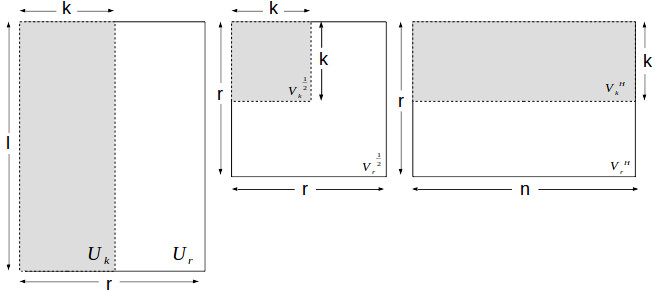
\includegraphics[scale=0.7]{figs/1.jpg}
\newline
\caption{Μείωση της διάστασης με \textlatin{SVD}} 
\end{figure}
\par
\vspace*{2cm}
Απο την παραπάνω ανάλυση καταλήγουμε στο συμπέρασμα ότι το \textlatin{l}-διάστατο διάνυσμα $ \mathbf{x}_{i} $ προσεγγίζεται απο το \textlatin{k}-διάστατο διάνυσμα $ \mathbf{a}_{i} $ που βρίσκεται στον υποχώρο που ορίζουν τα $ \mathbf{u}_{i},i=0,1,\ldots,k-1$ (το $ \mathbf{a}_{i}$ είναι στην ουσία η προβολή του $ \mathbf{x}_{i} $ στον υποχώρο αυτόν). Επίσης, λόγω της ορθοκανονικότητας των στηλών $ \mathbf{u}_{i},i=0,1,\ldots,k-1 $ του $ U_{k} $ βλέπουμε ότι
\newline\hspace*{\fill}
\begin{equation}
	\Vert \mathbf{x}_{i}-\mathbf{x}_{j} \Vert \simeq \Vert U_{k}(\mathbf{a}_{i}-\mathbf{a}_{j}) \Vert = \Vert \sum_{m=0}^{k-1} \mathbf{u}_{m} (a_{i}(m)-a_{j}(m)) \Vert = \Vert \mathbf{a}_{i}-\mathbf{a}_{j}\Vert, \quad i,j=0,1,\ldots,n-1
\end{equation}
\hspace*{\fill}\newline
Αντιλαμβανόμαστε λοιπόν ότι χρησιμοποιώντας την προηγούμενη προβολή και υποθέτοντας ότι η προσέγγιση είναι ικανοποιητική, η Ευκλείδεια απόσταση μεταξύ $ \mathbf{x}_{i} $ και $ \mathbf{x}_{j} $ στον υψηλής διάστασης $l$-διάστατο χώρο διατηρείται (κατά προσέγγιση) κατά την προβολή στον χαμηλότερης διάστασης $k$-διάστατο χώρο.
\section{Πρακτική εφαρμογή}
\par
Στο σημείο αυτό αξίζει να αναφερθεί ένα απλό παράδειγμα μέσω του οποίου μπορεί να γίνει αντιληπτή η πρακτική εφαρμογή των παραπάνω. Ας θεωρήσουμε λοιπόν ένα σύνολο $n$ προτύπων, όπου το καθένα αναπαρίσταται από ένα $l$-διάστατο διάνυσμα χαρακτηριστικών. Τότε, δοθέντος ενός άγνωστου προτύπου στόχος μας είναι να αναζητήσουμε στο σύνολο των γνωστών προτύπων που έχουμε ώστε να βρούμε αυτό το οποίο παρουσιάζει την μεγαλύτερη ομοιότητα με το άγνωστο για το οποίο θέλουμε να καταλήξουμε σε κάποιο συγκεκριμένο συμπέρασμα. Η διαδικασία αυτή είναι εφικτή υπολογίζοντας την Ευκλείδεια απόσταση μεταξύ του άγνωστου προτύπου με όλα τα γνωστά και επιλέγοντας τελικά το ζευγάρι με την μικρότερη απόσταση, δηλαδή αυτό με την μεγαλύτερη ομοιότητα.
\par
Σε περιπτώσεις όπου τόσο ο αριθμός των διαστάσεων όσο και ο αριθμός των δειγμάτων είναι μεγάλος τότε η παραπάνω διαδικασία μπορεί να είναι ιδιαίτερα χρονοβόρα. Προκειμένου λοιπόν να απλοποιήσουμε τους υπολογισμούς μπορούμε να ακολουθήσουμε την παραπάνω διαδικασία που αναλύσαμε ώστε να μειώσουμε τις διαστάσεις του προβλήματός μας. Η διαδικασία έχει ως εξής: Αρχικά σχηματίζουμε το μητρώο δεδομένων $X$, διάστασης $ l \times n $ με στήλες τα $n$ διανύσματα χαρακτηριστικών. Εκτελούμε την μεθοδολογία \textlatin{SVD}\textlatin{\cite{svd}\cite{13}} στο $X$ και αναπαριστούμε κάθε διάνυσμα χαρακτηριστικών $ \mathbf{x}_{i} $ με την χαμηλότερης διάστασης προβολή του, $ \mathbf{a}_{i} $. Το άγνωστο διάνυσμα προβάλλεται στον υποχώρο που ορίζουν οι στήλες του $U_{k}$ και εκτελούνται οι υπολογισμοί των Ευκλείδειων αποστάσεων στον $k$-διάστατο χώρο. Επειδή οι Ευκλείδειες αποστάσεις διατηρούνται κατά προσέγγιση, είναι εφικτό να αποφασίσουμε τους κοντινότερους γείτονες των διανυσμάτων εργαζόμενοι στον χώρο χαμηλότερης διάστασης. Σε περιπτώσεις για τις οποίες έχουμε $k \ll l$ επιτυγχάνεται σημαντική εξοικονόμηση στους υπολογισμούς.
\par
Τέλος, αξίζει να αναφερθεί ότι η μεθοδολογία \textlatin{SVD}\textlatin{\cite{svd}\cite{13}} είναι πολύ αποτελεσματική τεχνική μείωσης της διάστασης  σε περιπτώσεις όπου τα δεδομένα μπορούν να περιγραφούν επαρκώς μέσω του μητρώου συν διασποράς, για παράδειγμα περιπτώσεις όταν ακολουθούν κατανομές παρόμοιες με την \textlatin{Gaussian} κατανομή.





\chapter{Αλγόριθμοι μείωσης διαστάσεων}
\numberwithin{equation}{section}

\section{Γραμμική μείωση διαστάσεων}
\par
Όλες οι τεχνικές μείωσης διαστάσεων στις οποίες έχουμε αναφερθεί μέχρι στιγμής είναι κατεξοχήν τεχνικές μείωσης της διάστασης του χώρου των χαρακτηριστικών. Μάλιστα το ιδιαίτερο χαρακτηριστικό τους είναι ότι αποτελούν μεθόδους οι οποίες σέβονται την γραμμικότητα. Η μέθοδος \textlatin{PCA}\textlatin{\cite{pca}} για παράδειγμα η οποία αποτελεί μια απο τις γνωστότερες αλλά και πιο ισχυρές μεθόδους γραμμικής μείωσης διαστάσεων λειτουργεί καλά αν τα σημεία των δεδομένων είναι κατανεμημένα σε ένα υπερεπίπεδο. Όπως αναλύθηκε στην ενότητα (2.2) η μέθοδος \textlatin{PCA}\textlatin{\cite{pca}} προβάλλει στις διευθύνσεις μέγιστης διασποράς. Επίσης όπως εξηγήσαμε στο προηγούμενο κεφάλαιο η ανάλυση ιδιοτιμών-ιδιοδιανυσμάτων του μητρώου συσχέτισης αποκαλύπτει την διάσταση του υπέρ επιπέδου στο οποίο τα δεδομένα είναι διεσπαρμένα. 
\par
Με άλλα λόγια δηλαδή η διάσταση είναι ένα μέτρο του πλήθους των ελεύθερων μεταβλητών που είναι υπεύθυνες για τον τρόπο με τον οποίο μεταβάλλεται ένα σήμα, δηλαδή για την πραγματική πληροφορία την οποία κωδικοποιούν τα δεδομένα. 
\par
Παρότι ο αλγόριθμος \textlatin{PCA}\textlatin{\cite{pca}} αποτελεί μία πολύ ισχυρή και ευρέως χρησιμοποιούμενη μέθοδο μείωσης της διάστασης υπάρχουν περιπτώσεις στις οποίες η μέθοδος αποτυγχάνει. Τέτοιες είναι περιπτώσεις κατά τις οποίες ο μηχανισμός παραγωγής των δεδομένων είναι έντονα μη γραμμικός με αποτέλεσμα τα δεδομένα να κείτονται σε πιο περίπλοκες πολλαπλότητες. Ας πάρουμε για παράδειγμα τις εξισώσεις \\
\begin{center}
$x_{1}=r cos\theta, \quad x_{2}=rsin\theta$
\end{center}
Προφανώς απο τις παραπάνω εξισώσεις είναι φανερό ότι το $x$ βρίσκεται στην περιφέρεια κύκλου ακτίνας $r$. Πρόκειται δηλαδή για πρόβλημα μονοδιάστατης πολλαπλότητας αφού αρκεί μια μόνο μεταβλητή για την περιγραφή των δεδομένων. Η παράμετρος αυτή είναι η απόσταση κατα μήκος της περιφέρειας απο ένα σημείο(αφετηρία) πάνω στην περίμετρο του κύκλου. Αν λοιπόν εφαρμόσουμε την μέθοδο \textlatin{PCA}\textlatin{\cite{pca}} στο παραπάνω σύνολο δεδομένων τότε η απάντηση που θα μας δώσει για την διάσταση των δεδομένων θα είναι, λανθασμένα προφανώς, ίση με δύο. 
\par
Περιπτώσεις όπως οι παραπάνω απαιτούν αλγορίθμους μείωσης διάστασης και εξαγωγής χαρακτηριστικών οι οποίοι να λαμβάνουν υπόψιν την γεωμετρία του προβλήματος ώστε να μπορούν να εξάγουν ασφαλή συμπεράσματα για την διάσταση των δεδομένων. Στον τομέα της υπολογιστικής όρασης για παράδειγμα, ο οποίος όπως αναφέραμε και παραπάνω αποτελεί βασικό κομμάτι της εν λόγω διατριβής, απαιτούνται κατεξοχήν αλγόριθμοι μη γραμμικής μείωσης διαστάσεων αφού οι εικόνες ή τα χαρακτηριστικά των εικόνων τα οποία αποτελούν τα δεδομένα μας είναι κατά κύριο λόγο μη γραμμικά. 

\section{Μη γραμμική μείωση διαστάσεων}
\par
Υπάρχει λοιπόν μια ευρεία γκάμα εφαρμογών οι οποίες απαιτούν αλγορίθμους μη γραμμικής μείωσης διαστάσεων. Αυτό συμβαίνει διότι στις συγκεκριμένες εφαρμογές η γεωμετρική αναπαράσταση των δεδομένων είναι τέτοια ώστε απαιτείται να βρεθεί μια ενσωμάτωση μικρότερης διάστασης η οποία βρίσκεται <<κρυμμένη>> στον χώρο των αρχικών διαστάσεων. Θα πρέπει μάλιστα κατά την διαδικασία αυτή να ληφθούν υπόψιν τα γεωμετρικά χαρακτηριστικά του χώρου των δεδομένων. 
\par
Έχει πολύ μεγάλη σημασία στο σημείο αυτό να κατανοήσουμε τι εννοούμε όταν αναφερόμαστε στα γεωμετρικά χαρακτηριστικά του προβλήματος. Το πιο χαρακτηριστικό και ευρέως χρησιμοποιούμενο παράδειγμα για τον σκοπό αυτό είναι ένα τεχνητό σετ δεδομένων, με την όνομασία \textlatin{Swiss Roll}\textlatin{\cite{swiss_roll}} το οποίο φαίνεται στην παρακάτω εικόνα. \\
\vspace{1.0cm}
\begin{figure}[h]
\centering
%\hspace*{2.5cm}
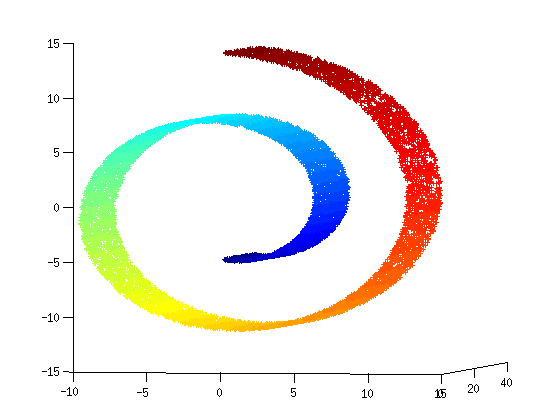
\includegraphics[scale=0.8]{figs/2.png}
\newline
\caption{ Τρισδιάστατη αναπαράσταση του συνθετικού σετ δεδομένων - \textlatin{Swiss Roll}.} 
\end{figure}
\vspace{1.0cm}
\par
Αυτό που αξίζει να παρατηρηθεί λοιπόν στο παραπάνω σετ δεδομένων είναι ότι αν για παράδειγμα διαλέξουμε κάποιο οποιοδήποτε σημείο του απο την κόκκινη περιοχή και προσπαθήσουμε να βρούμε ποια δεδομένα αποτελούν κοντινότερους γείτονες του σημείου αυτού πιθανότατα θα πέφταμε στην παγίδα, όπως και οι τεχνικές γραμμικής μείωσης διαστάσεων, να πούμε ότι κάποια σημεία από την μπλε περιοχή βρίσκονται και αυτά στην γειτονιά του σημείου που διαλέξαμε. Αυτό προφανώς είναι λάθος αφού από τον χρωματισμό των παραπάνω δεδομένων αντιλαμβανόμαστε ότι στην πραγματικότητα τα μπλε δεδομένα βρίσκονται πολύ μακριά από τα κόκκινα. Ο παραπάνω εσφαλμένος συλλογισμός αναπαρίσταται στο παρακάτω γράφημα.
\par
\begin{figure}[h!]
\centering
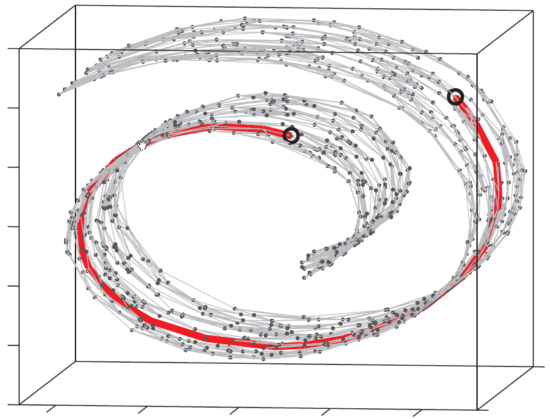
\includegraphics[scale=0.5]{figs/3.png}
\newline
\caption{Διάσχιση της γεωμετρίας - \textlatin{Swiss Roll}. (\textlatin{\cite{isomap}})} 
\end{figure}
\par
\vspace*{2cm}
Αντιλαμβανόμαστε λοιπόν, μέσω της παραπάνω απεικόνισης ότι θα πρέπει να ληφθεί υπόψιν η γεωμετρία του προβλήματος ώστε σε καμιά περίπτωση υπολογίζοντας κοντινότερες αποστάσεις να συμπεριλάβουμε το αρχικό και το τελικό σημείο ως κοντινούς γείτονες, ενώνοντάς τα απευθείας μεταξύ τους. Αυτή είναι και η διαφορά των αλγορίθμων μη γραμμικής μείωσης διαστάσεων με αυτούς της γραμμικής. Για να γίνει πλήρως κατανοητός ο τρόπος μείωσης των διαστάσεων του παραπάνω σετ δεδομένων, δίνεται η απεικόνιση των δεδομένων σε χώρο χαμηλής διάστασης μετά από την εφαρμογή αλγορίθμου μη γραμμικής μείωσης διαστάσεων.
\clearpage
\begin{figure}[t]
\centering
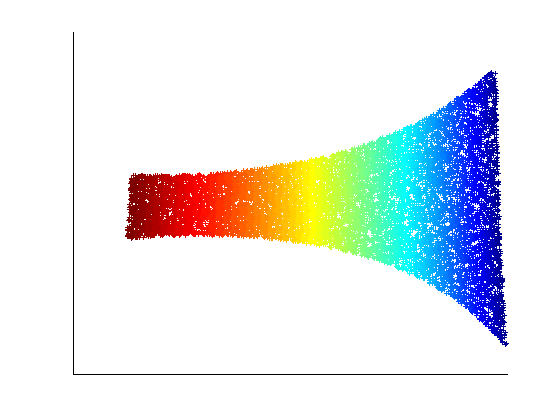
\includegraphics[scale=0.8]{figs/4.png}
\newline
\caption{Μείωση της διάστασης του \textlatin{Swiss Roll} απο τον τρισδιάστατο στον δυσδιάστατο χώρο.} 
\end{figure}
\par
\vspace*{1cm}
Απο την παραπάνω απεικόνιση μπορούμε να συμπεράνουμε ότι κάνοντας μείωση των διαστάσεων στην πραγματικότητα <<ξετυλίξαμε>> το \textlatin{Swiss Roll}\textlatin{\cite{swiss_roll}} και έτσι απο τον αρχικό χώρο των τριών διαστάσεων στην πραγματικότητα η εγγενής διάσταση των δεδομένων είναι ίση με δύο. Στις επόμενες ενότητες θα γίνει παρουσίαση των πιο γνωστών μεθόδων μη γραμμικής μείωσης διαστάσεων καθώς επίσης θα γίνει και η μαθηματική τους ανάλυση.


\subsection{\textlatin{ISOMAP}}
\par
Ένας βασικός αλγόριθμος μη γραμμικής μείωσης διαστάσεων είναι ο αλγόριθμος Ισομετρική απεικόνιση \textlatin{(Isometric Mapping - ISOMAP)}\textlatin{\cite{isomap}}. Ο αλγόριθμος αυτός υιοθετεί την άποψη ότι μόνο οι γεωδαιτικές αποστάσεις μεταξύ όλων των ζευγών των σημείων των δεδομένων μπορούν να αντικατοπτρίσουν την πραγματική δομή της πολλαπλότητας του προβλήματος. Η παραπάνω διατύπωση αντικατοπτρίζει το παράδειγμα που δόθηκε στο γράφημα (3.2), και τονίζει το γεγονός ότι οι Ευκλείδειες αποστάσεις μεταξύ σημείων μιας πολλαπλότητας δεν μπορούν να την αναπαραστήσουν ικανοποιητικά. Αυτό διότι σημεία (στο γράφημα τα δύο σημεία που έχουν επισημανθεί με μαύρους κύκλους) που είναι απομακρυσμένα μεταξύ τους σύμφωνα με την γεωδαιτική απόσταση, μπορεί να θεωρηθούν λανθασμένα, κοντινά ως προς την Ευκλείδεια απόστασή τους.
\par
Ουσιαστικά η μέθοδος \textlatin{ISOMAP}\textlatin{\cite{isomap}} είναι μια παραλλαγή του αλγορίθμου \textlatin{Multi Dimensional Scaling - MDS}\textlatin{\cite{mds}}, με την διαφορά ότι οι Ευκλείδειες αποστάσεις αντικαθίστανται από τις αντίστοιχες γεωδαιτικές κατά μήκος της πολλαπλότητας των δεδομένων. Η ουσία του αλγορίθμου είναι να εκτιμηθούν σωστά οι γεωδαιτικές αποστάσεις μεταξύ σημείων τα οποία είναι απομακρυσμένα μεταξύ τους. Ο αλγόριθμος μπορεί να χωριστεί σε δύο βασικά βήματα:
\par
\textbf{Βήμα-1}: \\ Για κάθε σημείο $x_{i},i=1,1\ldots,n$, υπολόγισε τους πλησιέστερους γείτονες και κατασκεύασε έναν γράφο $G(V,E)$ του οποίου οι κορυφές αναπαριστούν πρότυπα εισόδου και οι ακμές συνδέουν τους πλησιέστερους γείτονες. Οι παράμετροι $k$ (αριθμός των κοντινών γειτόνων κάθε σημείου) ή $\epsilon$ (ακτίνα σφαίρας στην οποία ανήκουν γειτονικά σημεία) είναι παράμετροι που καθορίζονται από τον χρήστη. Στις ακμές ανατίθενται βάρη σύμφωνα με τις αντίστοιχες Ευκλείδειες αποστάσεις (για τους πλησιέστερους γείτονες αυτή είναι μια καλή προσέγγιση της γεωδαιτικής απόστασης).
\par
\textbf{Βήμα-2}: \\ Υπολόγισε ανά ζεύγος την γεωδαιτική απόσταση για όλα τα ζεύγη κατά μήκος των συντομότερων διαδρομών μέσα στον γράφο. Το πιο σημαντικό σημείο, είναι ότι η γεωδαιτική απόσταση μεταξύ δύο οποιονδήποτε σημείων της πολλαπλότητας μπορεί να προσεγγιστεί μέσω της συντομότερης διαδρομής που ενώνει τα δύο σημείο στο γράφο $G(V,E)$. Ο πιο γνωστός αλγόριθμος υλοποίησης της παραπάνω διαδικασίας είναι ο αλγόριθμος \textlatin{Djikstar} με πολυπλοκότητα $\mathcal{O}(n^{2}\ln n + n^{2}k)$, μέγεθος απαγορευτικό για τις περισσότερες πρακτικές εφαρμογές.
\par
Εφόσον έχουν εκτελεστεί τα δύο αυτά βήματα είμαστε πλέον σε θέση νε εφαρμόσουμε την κλασική μέθοδο \textlatin{MDS}\textlatin{\cite{mds}}. Το πρόβλημα λοιπόν απο εδώ και στο εξής γίνεται ισοδύναμο με την εφαρμογή της ανάλυσης ιδιοδιανυσμάτων του αντίστοιχου μητρώου \textlatin{Gram} και την επιλογή των \textlatin{m} περισσότερο σημαντικών ιδιοδιανυσμάτων για την αναπαράσταση του χώρου χαμηλής διάστασης. Μετά απο αυτή την αναπαράσταση, οι Ευκλείδιες αποστάσεις μεταξύ των σημείων του χώρου χαμηλής διάστασης ταιριάζουν με τις αντίστοιχες γεωδαιτικές αποστάσεις στην πολλαπλότητα του αρχικού χώρου υψηλής διάστασης. Όπως και στις μεθόδους \textlatin{PCA}\textlatin{\cite{pca}} και \textlatin{MDS}\textlatin{\cite{mds}}. η διάσταση \textlatin{m} εκτιμάται απο το πλήθος των \textlatin{m} περισσότερο σημαντικών ιδιοτιμών. Αποδεικνύεται τέλος ότι η μέθοδος \textlatin{ISOMAP} ασυμπτωτικά ($n \rightarrow \inf$) θα ανακτήσει την αληθινή διάσταση για ένα σύνολο δεδομένων μη γραμμικής πολλαπλότητας.

\subsection{\textlatin{Laplacian Eigenmaps}}
\par
Η μέθοδος \textlatin{Laplassian Eigenmaps}\textlatin{\cite{laplassianeigenmaps}} στηρίζεται στην υπόθεση ότι τα σημεία των δεδομένων βρίσκονται σε μια λεία πολλαπλότητα $ Μ \supset Χ $, της οποίας η εγγενής διάσταση είναι ίση με $m<N$ και είναι ενσωματωμένη στον $ \Re^{N} $, δηλαδή $ Μ \supset \Re^{N} $. Η διάσταση $m$ δίνεται ως παράμετρος από τον χρήστη και εξαρτάται από το σύνολο των δεδομένων για κάθε εφαρμογή. Η κύρια φιλοσοφία πίσω από την μέθοδο είναι να υπολογιστεί η αναπαράσταση των δεδομένων σε χώρο χαμηλής διάστασης, έτσι ώστε η τοπική πληροφορία γειτνίασης στον χώρο $Χ \supset M$ να διατηρείται κατά βέλτιστο τρόπο. Με τον τρόπο αυτό προσπαθούμε να βρούμε μια λύση που αντανακλά τη γεωμετρική δομή της πολλαπλότητας. Για την επίτευξη αυτού απαιτούνται τα παρακάτω βήματα:
\par
\textbf{Βήμα-1}: Κατασκευή ενός γράφου $G=(V,E)$, όπου $V={v_{i},i=1,2,\ldots,n}$ είναι ένα σύνολο κορυφών και $E={\epsilon_{ij}}$ το σύνολο των ακμών που συνδέουν κορυφές $(v_{i},v_{j})$. Κάθε κόμβος $v_{i}$ του γράφου αντιστοιχεί σε ένα σημείο $\mathbf{x}_{i}$ του συνόλου των δεδομένων $X$. Συνδέουμε τις $v_{i}$,$v_{j}$, δηλαδή εισάγουμε την ακμή $\epsilon_{ij}$ μεταξύ των αντίστοιχων κόμβων, αν τα σημεία $\mathbf{x}_{i},\mathbf{x}_{j}$ είναι μεταξύ τους κοντινά. Η μέθοδος ορίζει την εγγύτητα αυτή με δύο τρόπους: \\
1. $\Vert \mathbf{x}_{i}-\mathbf{x}_{j} \Vert ^{2} < \epsilon $, για κάποια παράμετρο $\epsilon$ η οποία ορίζεται από τον χρήστη. Με $\Vert\cdot\Vert$ ορίζουμε την πράξη της Ευκλείδειας νόρμας στον χώρο $\Re^{N}$. \\
2. Το $\mathbf{x}_{j}$ είναι μεταξύ των $k$ πλησιέστερων γειτόνων του $\mathbf{x}_{i}$ ή και αντίστροφα, με το $k$ να είναι και σε αυτή την περίπτωση είσοδος η οποία καθορίζεται από τον χρήστη. Επίσης οι γείτονες επιλέγονται χρησιμοποιώντας την μετρική της Ευκλείδειας απόστασης στον χώρο $\Re^{N}$. Η χρήση της Ευκλείδειας απόστασης αιτιολογείται από την υπόθεση ότι η πολλαπλότητα είναι λεία, γεγονός που μας επιτρέπει να προσεγγίσουμε, τοπικά, τη γεωδαισία της πολλαπλότητας με Ευκλείδειες αποστάσεις.
\par
Για να αποσαφηνιστεί πλήρως η παραπάνω διατύπωση δίνεται το χαρακτηριστικό παράδειγμα όπου θεωρούμε μια σφαίρα ενσωματωμένη στον τρισδιάστατο χώρο, και έστω κάποιος περιορίζεται να ζει πάνω στην επιφάνεια της σφαίρας. Τότε η συντομότερη διαδρομή από ένα σημείο της σφαίρας σε ένα άλλο είναι η γεωδαιτική διαδρομή μεταξύ των δύο σημείων. Προφανώς αυτή δεν θα είναι ευθεία γραμμή, αλλά ένα τόξο στην επιφάνεια της σφαίρας. Παρόλα αυτά όμως, αν τα δύο σημεία είναι πολύ κοντά μεταξύ τους, η γεωδαιτική απόσταση μπορεί να προσεγγιστεί από την Ευκλείδεια απόσταση, υπολογισμένη στον τρισδιάστατο χώρο.
\par
\textbf{Βήμα-2}: Κάθε ακμή $\epsilon_{ij}$ συσχετίζεται με ένα βάρος $W(i,j)$. Για κόμβους που δεν συνδέονται μεταξύ τους, τα αντίστοιχα βάρη είναι μηδέν. Κάθε βάρος $W(i,j)$ είναι ένα μέτρο της εγγύτητας των αντίστοιχων γειτόνων $\mathbf{x}_{i},\mathbf{x}_{j}$. Μια τυπική επιλογή είναι \\
\newline\hspace*{\fill}
\[W(i,j) = \begin{cases} \exp(\Vert \frac{\mathbf{x}_{i}-\mathbf{x}_{j}}{\sigma^{2}} \Vert) \quad ,if \quad x_{i},x_{j} \quad neighbors\\
               0  \quad \quad \quad \quad \quad \quad ,not \quad neighbors\\
            \end{cases} \]
\hspace*{\fill}\newline 
με $\sigma^{2}$, παράμετρος η οποία ορίζεται και αυτή από τον χρήστη. Σχηματίζουμε το μητρώο βαρών $W$, μεγέθους ($n \times n$), το οποίο έχει για στοιχεία τα βάρη $W(i,j)$. Σημειώνουμε ότι το $W$ είναι συμμετρικό και αραιό αφού στην πράξη προκύπτει ότι πολλά από τα στοιχεία του είναι μηδενικά.
\par
\textbf{Βήμα-3}: Ορίζεται το διαγώνιο μητρώο $D$ με στοιχεία $D_{ij}=\sum_{j} W(i,j),i=1,2,\ldots,n,$ καθώς και το μητρώο $L=D-W$. Το τελευταίο είναι γνωστό ως το μητρώο \textlatin{Laplace} του γράφου $G=(V,E)$. Εφαρμόζεται η γενικευμένη ανάλυση σε ιδιοτιμές και ιδιοδιανύσματα 
\newline\hspace*{\fill}
$ \Lambda \mathbf{v} =  \lambda D \mathbf{v} $
\hspace*{\fill}\newline 
Έστω $ 0 = \lambda_{0} \leq \lambda_{1} \leq \lambda_{2} \leq \ldots \leq \lambda_{m}$, οι $m+1$ μικρότερες ιδιοτιμές. Αγνοείται η ιδιοτιμή $\mathbf{v}_{0}$ που αντιστοιχεί στην ιδιοτιμή $\lambda_{0} = 0$ και επιλέγονται τα υπόλοιπα $m$ ιδιοδιανύσματα $\mathbf{v}_{1},\mathbf{v}_{2},\ldots,\mathbf{v}_{m},$. Στην συνέχεια εκτελείται η απεικόνιση
\newline\hspace*{\fill}
$\mathbf{x}_{i} \in \Re^{N} \mapsto \mathbf{y}_{i} \in \Re^{m}, i=1,2,\ldots,n$
\hspace*{\fill}\newline 
όπου 
\newline\hspace*{\fill}
$\mathbf{y}_{i}^{T} = [\mathbf{v}_{1}(i),\mathbf{v}_{2}(i),\ldots,\mathbf{v}_{m}(i)], i=1,2,\ldots,m$
\hspace*{\fill}\newline
\par
Όπως έχουμε αναλύσει στην αντίστοιχη εντότητα η πολυπλοκότητα υπολογισμού ιδιοτιμών και ιδιοδιανυσμάτων είναι, γενικά, της τάξης $\mathcal{O}(n^{3})$. Ωστόσο για αραιά μητρώα, όπως στην συγκεκριμένη περίπτωση το $L$, μπορούν να εφαρμοστούν αποτελεσματικές τεχνικές με αποτέλεσμα την μείωση της πολυπλοκότητας σε τάξη κάποιο πολλαπλάσιο του $\mathcal{O}(n^2)$. Η πιο γνωστή και αποτελεσματική τεχνική για τον σκοπό αυτό είναι ο αλγόριθμος \textlatin{Lanczos}\textlatin{\cite{lanczos}}.
\par
Ο αλγόριθμος \textlatin{Laplassian Eigenmaps}\textlatin{\cite{laplassianeigenmaps}} ο οποίος αναλύθηκε παραπάνω, ανήκει στην ίδια κατηγορία (\textit{μέθοδοι μείωσης διαστάσεων που βασίζονται σε γράφους}) με τον αλγόριθμο \textbf{\textlatin{Locally Linear Embeddings - LLE}}\textlatin{\cite{lle}} ο οποίος αποτελεί και βασικό αντικείμενο της εν λόγω διατριβής. Οι δύο αλγόριθμοι έχουν πολύ κοινή λογική και μεθοδολογία και γι αυτό στο επόμενο κεφάλαιο στο οποίο γίνεται αναλυτική μαθηματική ανάλυση του \textlatin{LLE}\textlatin{\cite{lle}} θα αποσαφηνιστούν και τα παραπάνω βήματα του \textlatin{Laplassian Eigenmaps}\textlatin{\cite{laplassianeigenmaps}} καθώς τα βήματα τους είναι πανομοιότυπα.



\chapter{Τοπική Γραμμική Ενσωμάτωση (\textlatin{Locally Linear Embeddings - LLE})}
\numberwithin{equation}{section}
\par
Ο αλγόριθμος \textlatin{Locally Linear Embeddings (LLE)}\cite{lle} ανήκει στην κατηγορία αλγορίθμων μη γραμμικής μείωσης διαστάσεων με την χρήση γράφων και αποτελεί μια από τις αποτελεσματικότερες αλλά και γρηγορότερες τεχνικές αυτού του είδους. Όπως αναφέραμε και στο προηγούμενο κεφάλαιο, βασική υπόθεση της μεθόδου είναι ότι τα δεδομένα μας βρίσκονται σε μια αρκετά λεία πολλαπλότητα, διάστασης $m$, και η οποία είναι ενσωματωμένη στον υποχώρο του $ \Re^{N} $, με $m<N$. Η υπόθεση για το λείο της πολλαπλότητας μας επιτρέπει να υποθέσουμε επιπλέον ότι, με δεδομένη την ύπαρξη αρκετών δεδομένων και ότι η πολλαπλότητα είναι <<καλά>> δειγματοληπτημένη, τα κοντινά σημεία βρίσκονται πάνω (ή κοντά) σε ένα <<τοπικό>> γραμμικό τμήμα της πολλαπλότητας.

\section{Ο αλγόριθμος ως τεχνική μη γραμμικής μείωσης διαστάσεων}
\par
Δεδομένης της αποτελεσματικότητας του αλγορίθμου να ανακαλύπτει τον χώρο μειωμένης διάστασης στον οποίο βρίσκεται ενσωματωμένη η πληροφορία ενός προβλήματος, ο αλγόριθμος έχει χρησιμοποιηθεί με επιτυχία σε αρκετές πρακτικές εφαρμογές. Ιδιαίτερο ενδιαφέρον παρουσιάζουν νέες μελέτες κυρίως απο τον χώρο της Ιατρικής \cite{1} \cite{2}. Απο τις αναφορές αυτές είναι φανερό ότι ο ρόλος της μείωσης των διαστάσεων μπορεί να καθορίσει σε μεγάλο βαθμό την βελτίωση του αποτελέσματος ταξινόμησης. Στις συγκεκριμένες περιπτώσεις στόχος είναι να γίνει σωστή πρόβλεψη για το αν κάποιος ασθενής πάσχει απο μια συγκεκριμένη ασθένεια ή βρίσκεται στην ευπαθή ομάδα με μεγάλη πιθανότητα να του παρουσιαστεί στο μέλλον. Φαίνεται οτι ο αλγόριθμος \textlatin{LLE}\textlatin{\cite{lle}} είναι ένα πολύ ισχυρό εργαλείο το οποίο μπορεί να υλοποιήσει την μείωση των διαστάσεων σε τέτοιου είδους εφαρμογές και μάλιστα επιφέροντας σημαντικά και ουσιαστικά αποτελέσματα. Ο αλγόριθμος επίσης, έχει χρησιμοποιηθεί και σε εφαρμογές ταξινόμησης με σετ δεδομένων ευρέως διαδεδομένα στον χώρο της αναγνώρισης προτύπων \cite{3} \cite{4} \cite{5}, όπως το σετ δεδομένων με χειρόγραφα ψηφία \textlatin{MNIST}\textlatin{\cite{mnist}}.

\section{Μαθηματική ανάλυση και υλοποίηση του αλγορίθμου \textlatin{Locally Linear Embeddings}}
\par
Ο αλγόριθμος \textlatin{LLE}\cite{lle} αποτελεί το κύριο κομμάτι της εν λόγω διατριβής και η υλοποίηση του έχει στηριχθεί στον αλγόριθμο της παραπάνω αναφοράς. Ο ψευδοκώδικας είναι διαθέσιμος στον παρακάτω σύνδεσμο: \href{https://www.cs.nyu.edu/~roweis/lle/algorithm.html}{\textlatin{LLE Algorithm Pseudocode}}. Παρ' όλα αυτά στην συγκεκριμένη υλοποίηση έχουν γίνει συγκεκριμένες βελτιστοποιήσεις σε κάποια βήματα του αλγορίθμου, όπως για παράδειγμα η χρήση του \href{http://autogpu.ee.auth.gr/doku.php?id=cuknns:gpu_accelerated_k-nearest_neighbor_library}{αλγορίθμου κοντινότερων γειτόνων \textlatin{(k-NN)} υλοποιημένο σε \textlatin{CUDA}}, με σκοπό την μείωση του χρόνου εκτέλεσης του συγκεκριμένου βήματος. 

\subsection{Βήμα-1: Εύρεση του πίνακα γειτνίασης}
\par
Κατά το πρώτο βήμα του αλγορίθμου γίνεται ο υπολογισμός των κοντινότερων γειτόνων για κάθε σημείο $X_{i}$ του συνόλου των δεδομένων. Στο βήμα αυτό ο χρήστης επιλέγει ανάλογα με την κάθε εφαρμογή έναν αριθμό γειτόνων \textlatin{K} και χρησιμοποιεί κάποιον αλγόριθμο υπολογισμού κοντινότερων γειτόνων για κάθε ένα από τα σημεία του δείγματος. Με τον τρόπο αυτό έχει υπολογιστεί ο τετραγωνικός πίνακας $N \times N$, ο οποίος δίνει πληροφορία για κάθε σημείο του δείγματος ως προς τους \textlatin{k} κοντινότερους γείτονές του.
\par
Ο τρόπος υπολογισμού του πίνακα αυτού στην συγκεκριμένη υλοποίηση γίνεται μέσω της συνάρτησης \textlatin{knnsearch} του \textlatin{MATLAB} για την σειριακή υλοποίηση και με την συνάρτηση \textlatin{gpu\textunderscore knn} για την παράλληλη υλοποίηση. Η συνάρτηση αυτή αντιπροσωπεύει την κύρια συνάρτηση \textlatin{gpuknnHeap} του πακέτου \href{http://autogpu.ee.auth.gr/doku.php?id=cuknns:gpu_accelerated_k-nearest_neighbor_library}{\textlatin{knn-toolbox}}, η οποία με την σειρά της αποτελεί το πέρασμα απο τον κώδικα \textlatin{MATLAB} στην συνάρτηση πυρήνα υπολογισμού κοντινότερων γειτόνων με τη χρήση παράλληλης υλοποίησης σε \textlatin{CUDA} γραμμένη στην γλώσσα προγραμματισμού \textlatin{C}. Η υλοποίηση αυτή χρησιμοποιεί την Ευκλείδεια απόσταση ως μέθοδο προσδιορισμού των κοντινότερων γειτόνων. Παρ' όλα αυτά στο βήμα αυτό μπορούν να χρησιμοποιηθούν και άλλες μετρικές γειτνίασης όπως για παράδειγμα ο προσδιορισμός κοντινών γειτόνων με τη χρήση σφαίρας ακτίνας $\epsilon$. Επίσης, μια άλλη γνωστή μέθοδος επίλυσης του βήματος αυτού η οποία βελτιώνει τον χρόνο εκτέλεσης είναι η χρήση %\href{https://en.wikipedia.org/wiki/K-d_tree}
{\textlatin{KD-trees}}.

\subsection{Βήμα-2: Εύρεση του πίνακα βαρών \textlatin{W}}
\par
Στο δεύτερο αυτό βήμα του αλγορίθμου στόχος είναι να υπολογιστεί ο πίνακας βαρών $W(i,j),i,j=1,2,\ldots,n,$ μέσω των οποίων είναι εφικτή η ανακατασκευή του κάθε δείγματος $X_{i}$ μέσω των βαρών που αντιστοιχούν στους κοντινότερους γείτονές του. Πιο απλά στο βήμα αυτό θέλουμε να προσδιορίζουμε κάθε σημείο $X_{i}$ του δείγματός μας, ελαχιστοποιώντας την συνάρτηση κόστους
\newline\hspace*{\fill}
\begin{equation}
        \arg \min_{w} E_{w} = \sum_{i=1}^{n} \Vert \mathbf{X_{i}} - \sum_{j=1}^{n} W(i,j)\mathbf{X}_{j} \Vert ^{2}
\end{equation}
\hspace*{\fill}\newline
η οποία στην πραγματικότητα αυτό που προσπαθεί να ανακαλύψει είναι οι κοντινότεροι γείτονες $j$ του σημείου $X_{i}$ οι οποίοι ασκούν την σημαντικότερη επιρροή πάνω του ως προς την ανακατασκευή του. Η ελαχιστοποίηση της συνάρτησης αυτής γίνεται εφαρμόζοντας τον αλγόριθμο ελαχίστων τετραγώνων %\href{https://en.wikipedia.org/wiki/Least_squares}
({\textlatin{Least squares}}) εξασφαλίζοντας παράλληλα κάποιες απαραίτητες ιδιότητες για τον πίνακα βαρών $W$. Καταρχήν πρέπει να ισχύει ότι το κάθε δείγμα $X_{i}$ θα πρέπει να μπορεί να ανακατασκευαστεί μόνο απο τους κοντινότερους γείτονές του γεγονός που θέτει τον περιορισμό $W(i,j)=0$ στην περίπτωση κατά την οποία το $j$ στοιχείο δεν είναι γείτονας του $i$. Επίσης θα πρέπει τα στοιχεία κάθε γραμμής του μητρώου βαρών $W$ να αθροίζονται στην μονάδα, δηλαδή $\sum_{j=1}^{n} W(i,j)=1$, ώστε να εξασφαλιστεί η αμεταβλητότητα κατά την μεταφορά. Με τους περιορισμούς αυτούς λοιπόν εξασφαλίζεται ότι τα βάρη τα οποία ελαχιστοποιούν την παραπάνω συνάρτηση κόστους είναι αμετάβλητα κατά την περιστροφή, την μεταφορά και την κλιμάκωση.
\par
%Η παραπάνω διαδικασία υλοποιείται με τον παρακάτω κώδικα σε 
%\textlatin{MATLAB}.
%\selectlanguage{english}
%\begin{lstlisting}[language=Matlab]
%W = zeros(K,N);
%for ii=1:N
%   z = X(:,neighborhood(:,ii))-repmat(X(:,ii),1,K); 
%   C = z'*z;                                        % local covariance
%   C = C + eye(K,K)*tol*trace(C);                   % regularlization (K>D)
%   W(:,ii) = C\ones(K,1);                           % solve Cw=1
%   W(:,ii) = W(:,ii)/sum(W(:,ii));                  % enforce sum(w)=1
%end;
%\end{lstlisting}
%\selectlanguage{greek}
Για να γίνει κατανοητή η παραπάνω διαδικασία ακολουθούμε τον εξής συλλογισμό. Ας πάρουμε για παράδειγμα ένα σημείο $x$ το οποίο έχει $K$ κοντινούς γείτονες $n_{j}$ και βάρη ανακατασκευής $w_{j}$ για τα οποία ισχύει η συνθήκη $\sum_{j} w_{j} = 1$. Τότε μπορούμε να γράψουμε την συνάρτηση κόστους ως
\newline\hspace*{\fill}
\begin{equation}
        \epsilon = \mid \overrightarrow{x} - \sum_{j} w_{j}\overrightarrow{n}_{j} \mid ^{2} = \mid \sum_{j} w_{j}(\overrightarrow{x}-\overrightarrow{n}_{j}) \mid ^{2} = \sum_{jk} w_{j}w_{k}C_{jk}
\end{equation}
\hspace*{\fill}\newline
Στην παραπάνω σχέση χρησιμοποιήσαμε το μητρώο \textlatin{Gram} το οποίο ορίζεται ως
\newline\hspace*{\fill}
\begin{equation}
        C_{jk} = (\overrightarrow{x}-\overrightarrow{n}_{j})
        \cdot(\overrightarrow{x}-\overrightarrow{n}_{k})
\end{equation}
\hspace*{\fill}\newline
Εκ κατασκευής για τον πίνακα \textlatin{Gram} έχουμε ότι είναι συμμετρικός και θετικά ημιορισμένος. Σύμφωνα με τα παραπάνω λοιπόν τα βέλτιστα βάρη ανακατασκευής $w_{j}$ της συνάρτησης κόστους μπορούν να υπολογιστούν, αφού μέσω του πολλαπλασιαστή \textlatin{Lagrange} εξασφαλίσουμε τη συνθήκη $\sum_{j} w_{j} = 1$, μέσω της επίλυσης του συστήματος
\newline\hspace*{\fill}
\begin{equation}
	w_{j} = \dfrac{\sum_{k}C_{jk}^{-1}}{\sum_{lm}G_{lm}^{-1}}
\end{equation}
\hspace*{\fill}\newline
Όπως είχαμε αναφέρει στην παράγραφο (2.3) οι πίνακες $X^{T}X$(πίνακας συνδιασποράς) και $XX^{T}$(πίνακας \textlatin{Gram}) έχουν τις ίδιες ιδιοτιμές και ιδιοδιανύσματα τα οποία σχετίζονται μεταξύ τους. Για τον λόγο αυτό μπορεί να παραληφθεί η αντιστροφή του πίνακα \textlatin{Gram}, όπως φαίνεται και στην υλοποίηση που παρατέθηκε παραπάνω, λύνοντας το σύστημα $\sum_{j}C_{jk}w_{k}=1$ και έπειτα απαιτώντας τον περιορισμό $\sum_{j} w_{j}=1$ ο οποίος υλοποιείται με την τελευταία γραμμή του παραπάνω κώδικα. Επίσης βλέπουμε ότι στην υλοποίηση του κώδικα δεν υπολογίζεται ο πίνακας \textlatin{Gram} αλλά αυτός της συνδιασποράς και στην συνέχεια ακολουθείται η παραπάνω διαδικασία. Τελευταία διευκρίνηση για τη γραμμή 5 του κώδικα, στην οποία γίνεται κανονικοποίηση του πίνακα συνδιασποράς. Αυτό απαιτείται στην περίπτωση για την οποία ο πίνακας συνδιασποράς προκύπτει μοναδιαίος ή πολύ κοντά σε αυτόν, οπότε και δεν υπάρχει μοναδική λύση του συστήματος.
\par
Καταλήγουμε λοιπόν μέσω της παραπάνω διαδικασίας στον υπολογισμό του μητρώου βαρών \textlatin{W} για το σύνολο των δεδομένων. Ο τρόπος μάλιστα με τον οποίο έγινε ο υπολογισμός αυτός εξασφαλίζει το γεγονός ότι η εσωτερική ενσωματωμένη γεωμετρία η οποία υπάρχει στην γειτονιά ενός σημείου $X_{i}$ του συνόλου των δεδομένων θα εξακολουθεί να υπάρχει και στον χώρο της μειωμένης διάστασης. Το γεγονός αυτό εξασφαλίζεται από την ανεξαρτησία των βαρών ως προς την περιστροφή, την μεταφορά και την κλιμάκωση αλλά και από το γεγονός ότι οι γείτονες του σημείου $X_{i}$ στον χώρο αρχικών διαστάσεων $D$ θα εξακολουθούν να αποτελούν γείτονες του σημείου $Y_{i}$ (προβολή του $X_{i}$ από τον χώρο υψηλής διάστασης στο σημείο $Y_{i}$ χαμηλής διάστασης). Αυτό συμβαίνει επίσης, διότι όπως θα δούμε παρακάτω τα βάρη με τα οποία γίνεται ανακατασκευή του $X_{i}$ τα ίδια θα χρησιμοποιηθούν και για την κατασκευή του $Y_{i}$ στον χώρο μειωμένης διάστασης. Συνέπεια λοιπόν των παραπάνω είναι ότι τα βάρη $w_{j}$ που υπολογίστηκαν δεν εξαρτώνται από το εκάστοτε σημείο αλλά κωδικοποιούν πληροφορία σχετική με τα εγγενή χαρακτηριστικά κάθε γειτονιάς τα οποία και διατηρούνται κατά την ενσωμάτωση των δεδομένων στον χώρο χαμηλότερης διάστασης. 

\subsection{Βήμα-3: Επιλογή των τελικών διαστάσεων με τη χρήση του πίνακα \textlatin{W}}
\par
Στο τελευταίο βήμα του αλγορίθμου πραγματοποιείται η μείωση των διαστάσεων των δειγμάτων από τον χώρο υψηλής διάστασης $D$ σε έναν χαμηλότερης $d$. Η διαδικασία αυτή πραγματοποιείται όπως αναφέραμε και παραπάνω χρησιμοποιώντας τον πίνακα των βαρών $W$ και τα οποία έχουν την ιδιότητα ότι αντανακλούν τις εγγενείς ιδιότητες της τοπικής γεωμετρίας στην οποία υπόκεινται τα δεδομένα. Η λύση λοιπόν προκύπτει επιλύοντας και πάλι ένα πρόβλημα ελαχιστοποίησης το οποίο ορίζεται ως
\newline\hspace*{\fill}
\begin{equation}
        \arg \min_{w} E_{y} = \sum_{i=1}^{n} \Vert \mathbf{Y_{i}} - \sum_{j=1}^{n} W(i,j)\mathbf{Y}_{j} \Vert ^{2}
\end{equation}
\hspace*{\fill}\newline
Και σε αυτή την περίπτωση  απαιτούμε την διατήρηση των συνθηκών, $\sum_{i} Y_{i} = 0$ ώστε να εξασφαλιστεί η αμεταβλητότητα ως προς την μεταφορά, και $ \dfrac{1}{N} \sum_{i} Y_{i}Y{i}^{T} = I $ η οποία εξασφαλίζει ότι οι διαστάσεις $d$ θα είναι δευτέρου βαθμού ασυσχέτιστες , ότι τα βάρη ανακατασκευής για τις διαστάσεις $d$ θα υπολογιστούν σε κοινή κλίμακα και ότι αυτή η κλίμακα θα είναι μοναδιαίου βαθμού. Ο πίνακας $I$ συμβολίζει τον μοναδιαίο πίνακα διάστασης $d \times d$. 
\par
Η λύση της εξίσωσης (4.2.5) για τα άγνωστα στοιχεία $y_{i},i=1,2,\ldots,n$, είναι ισοδύναμη με την εύρεση των $d+1$ μικρότερων ιδιοτιμών του τετραγωνικού πίνακα $M$ ο οποίος προκύπτει από την σχέση
\newline\hspace*{\fill}
\begin{equation}
        E_{y} = \sum_{i=1}^{n} \Vert \mathbf{Y_{i}} - \sum_{j=1}^{n} W(i,j)\mathbf{Y}_{j} \Vert ^{2} = \mid (I-W)Y \mid ^{2} = Y_{T}MY
\end{equation}
\hspace*{\fill}\newline
και ισούτε με
\begin{equation}
        M = (I-W)^{T}(I-W)
\end{equation}
\hspace*{\fill}\newline
Ο πίνακας αυτός έχει διαστάσεις $N \times N$, όπου $N$ το πλήθος των δεδομένων εισόδων. Παρόλα αυτά ο πίνακας αυτός στην πράξη προκύπτει αραιός \textlatin{(sparce matrix)} γεγονός το οποίο απλοποιεί σημαντικά τους υπολογισμούς, ιδιαίτερα για μεγάλες τιμές του $N$. Στην συνέχεια χρησιμοποιώντας τον πολλαπλασιαστή \textlatin{Lagrange} καταλήγουμε στην επίλυση της εξίσωσης
\begin{equation}
        (M-\Lambda)Y^{T} = 0
\end{equation}
\hspace*{\fill}\newline
όπου $\Lambda$ είναι ο διαγώνιος πίνακας των πολλαπλασιαστών \textlatin{Lagrange}. 
%Η υλοποίηση της παραπάνω διαδικασίας στην συγκεκριμένη υλοποίηση σε κώδικα \textlatin{MATLAB} είναι η παρακάτω
%\selectlanguage{english}
%\begin{lstlisting}[language=Matlab]
% M=eye(N,N); % use a sparse matrix with storage for 4KN nonzero elements
%M = sparse(1:N,1:N,ones(1,N),N,N,4*K*N); 
%for ii=1:N
%   w = W(:,ii);
%   jj = neighborhood(:,ii);
%   M(ii,jj) = M(ii,jj) - w';
%   M(jj,ii) = M(jj,ii) - w;
%   M(jj,jj) = M(jj,jj) + w*w';
%end;
%\end{lstlisting}
%\selectlanguage{greek}
\par
Η παραπάνω επίλυση του προβλήματος ανάλυσης ιδιοτιμών μας οδηγεί στον προσδιορισμό των ιδιοδιανυσμάτων τα οποία αποτελούν και λύσεις του πίνακα $M$. Επίσης τα ιδιοδιανύσματα με τις μεγαλύτερες ιδιοτιμές είναι αυτά τα οποία ελαχιστοποιούν την συνάρτηση κόστους την οποία και θέλαμε να επιλύσουμε. Στο σημείο αυτό λοιπόν είμαστε σε θέση να προσδιορίσουμε τις τελικές διαστάσεις οι οποίες αντιπροσωπεύουν τα δεδομένα μας στον νέο χώρο μειωμένης διάστασης. Οι τελικές αυτές διαστάσεις $d$ λαμβάνουν υπόψιν τους περιορισμούς οι οποίοι έχουν τεθεί και έτσι με τον τρόπο αυτό εξασφαλίζεται η διατήρηση των γεωμετρικών χαρακτηριστικών της κάθε γειτονιάς για όλα τα σημεία $X_{i}$ του αρχικού συνόλου δεδομένων μεγέθους $N$. 
\par
Σημαντικό σημείο στην παραπάνω διαδικασία αποτελεί το γεγονός ότι δεν λαμβάνουμε υπόψιν την μικρότερη ιδιοτιμή της λύσης του παραπάνω συστήματος και αυτό διότι ισούται με το μηδέν. Η ιδιοτιμή αυτή αντιπροσωπεύει το μοναδιαίο διάνυσμα το οποίο εξασφαλίζει ότι το σύνολο των δεδομένων έχει μηδενική μέση τιμή, εξασφαλίζοντας έτσι τον περιορισμό ως προς την αμεταβλητότητα κατά την μεταφορά.
\par
%Η παραπάνω διαδικασία απόρριψης την μηδενικής ιδιοτιμής και τελικά της επιλογής των τελικών διαστάσεων οι οποίες και αντιπροσωπεύουν τα αρχικά δεδομένα στον χώρο μειωμένης διάστασης υλοποιούνται με τον παρακάτω κώδικα \textlatin{MATLAB}
%\selectlanguage{english}
%\begin{lstlisting}[language=Matlab]
%options.disp = 0; options.isreal = 1; options.issym = 1; 
%[Y,eigenvals] = eigs(M,d+1,0,options);
%
%Y = Y(:,end-1:-1:end-d)'*sqrt(N); % bottom evect is [1,1,1,1...] with eval 0
%\end{lstlisting}
%\selectlanguage{greek}
Η εύρεση των ιδιοτιμών-ιδιοδιανυσμάτων γίνεται με τον αλγόριθμο \textlatin{Lanczos}\textlatin{\cite{lanczos}} ο οποίος βελτιστοποιεί σε μεγάλο βαθμό την επίλυση του προβλήματος, από την στιγμή που ο τετραγωνικός πίνακας $M$ του συστήματος είναι αραιός και θετικά ημιορισμένος και η επίλυση γίνεται για τις \textlatin{d} κοντινότερες στο μηδέν ιδιοτιμές.


%\addcontentsline{toc}{chapter}{Συμπεράσματα}

\chapter{Συμπεράσματα}

\section{Συμπεράσματα για τα πειράματα}

\section{Συμπεράσματα για τον αλγόριθμο \textlatin{Locally Linear Embeddings}}

\section{Συμπεράσματα για την μείωση διαστάσεων σε αφαρμογές μηχανικής μάθησης και εξόρυξης γνώσης}


\appendix
% appendices come here


\addcontentsline{toc}{chapter}{Βιβλιογραφία}
\bibliographystyle{alpha}
\bibliography{bibliography/bibliography}

\end{document}
